\documentclass[a4paper]{article}
\usepackage[T1]{fontenc}			% pacchetto per \chapter
\usepackage[italian]{babel}
\usepackage[italian]{isodate}  		% formato delle date in italiano
\usepackage{graphicx}				% gestione delle immagini
\usepackage{amsfonts}
\usepackage{booktabs}				% tabelle di qualità superiore
\usepackage{amsmath}				% pacchetto matematica
\usepackage{mathtools}				% per sottolineare sotto le equazioni
\usepackage{stmaryrd} 				% per '\llbracket' e '\rrbracket'
\usepackage{amsthm}					% teoremi migliorati
\usepackage{enumitem}				% gestione delle liste
\usepackage{pifont}					% pacchetto con elenchi carini
\usepackage{cancel}					% per cancellare delle espressioni matematiche
\usepackage{caption}				% caption personalizzati
\usepackage[]{mdframed}				% box per il testo
\usepackage{multirow}				% più linee in una tabella
\usepackage{gensymb}				% simbolo di degree
\usepackage[x11names]{xcolor}		% pacchetto colori RGB
\usepackage{tcolorbox}				% pacchetto per le box colorate

% draw a frame around given text
\newcommand{\framedtext}[1]{%
	\par%
	\noindent\fbox{%
		\parbox{\dimexpr\linewidth-2\fboxsep-2\fboxrule}{#1}%
	}%
}


% Link ipertestuali per l'indice
\usepackage{xcolor}
\usepackage[linkcolor=black, citecolor=blue, urlcolor=cyan]{hyperref}
\hypersetup{
	colorlinks=true
}

\usepackage{tikz}
\newcommand{\MyTikzmark}[2]{%
	\tikz[overlay,remember picture,baseline] \node [anchor=base] (#1) {#2};%
}
\newcommand{\DrawVLine}[3][]{%
	\begin{tikzpicture}[overlay,remember picture]
		\draw[shorten <=0.3ex, #1] (#2.north) -- (#3.south);
	\end{tikzpicture}
}
\newcommand{\DrawHLine}[3][]{%
	\begin{tikzpicture}[overlay,remember picture]
		\draw[shorten <=0.2em, #1] (#2.west) -- (#3.east);
	\end{tikzpicture}
}


%\usepackage{showframe}				% visualizzazione bordi
%\usepackage{showkeys}				% visualizzazione etichetta

\newtheorem{theorem}{\textcolor{Red3}{\underline{Teorema}}}
\newtheorem{lemma}{Lemma}
\renewcommand{\qedsymbol}{QED}
\newcommand{\exec}[1]{\llbracket #1\:\rrbracket}
\newcommand{\dquotes}[1]{``#1''}
\newcommand{\longline}{\noindent\rule{\textwidth}{0.4pt}}
\newcommand{\circledtext}[1]{\raisebox{.5pt}{\textcircled{\raisebox{-.9pt}{#1}}}}
\newcommand{\definition}[1]{\textcolor{Red3}{\textbf{#1}}}
\newcommand{\example}[1]{\textcolor{Green4}{\textbf{#1}}}

\newenvironment{rowequmat}[1]{\left(\array{@{}#1@{}}}{\endarray\right)}
\newenvironment{rowequmatbra}[1]{\left[\array{@{}#1@{}}}{\endarray\right]}

\begin{document}
	\newcounter{definition}[section]
	\newtcolorbox{boxdef}{colback=red!5!white,colframe=red!75!black,fonttitle=\bfseries,title=Definizione~\refstepcounter{definition}\thedefinition}

	\author{VR443470}
	\title{Schemi Analisi II}
	\date{\printdayoff\today}
	\maketitle
	
	\newpage
	
	% indice
	\tableofcontents
	
	\newpage
	
	%%%%%%%%%%%%%%%%
	% Prerequisiti %
	%%%%%%%%%%%%%%%%
	\section{Prerequisiti}\label{section: prerequisiti}
	
	Il corso di Analisi II si articola in due macro sezioni: primo e secondo parziale. All'esame gli esercizi da svolgere saranno 10, suddivisi 5 per la prima parte e 5 per la seconda.\newline
	
	\noindent
	Nonostante vengano date 3 ore per svolgere l'esame totale, dunque 1 ora e mezza per ciascuna prova parziale, il tempo è una risorsa fondamentale. Difatti, se un calcolo matematico dovesse richiedere una quantità eccessiva di risorse/tempo, si rischierebbe di non passare l'esame con esito positivo.\newline
	
	\noindent
	Risulta dunque fondamentale, per ciascun studente, giungere con dei prerequisiti solidi e non banali. In questo capitolo si provvederà a fornire alcuni prerequisiti necessari per affrontare il percorso senza eccessive difficoltà.\newline
	
	\noindent
	Ogni paragrafo presenterà degli esercizi e ognuno di essi sarà risolto nel seguente modo: il primo in modo approfondito per illustrare il modus operandi, gli altri facendo vedere i calcoli e risparmiando le spiegazioni prolisse. Chiaramente, nel caso in cui ci dovesse essere un caso particolare, esso verrà affrontato e spiegato passo passo.\newpage
	
	%%%%%%%%%%%%%%%%%%%%%%%
	% Geometria analitica %
	%%%%%%%%%%%%%%%%%%%%%%%
	\subsection{Geometria analitica}\label{subsection: geometria analitica}
	
	%%%%%%%%%%%%%%%%%
	% Circonferenza %
	%%%%%%%%%%%%%%%%%
	\subsubsection{Circonferenza}\label{subsubsection: circonferenza}
	
	La circonferenza è graficamente rappresentata nel seguente modo:
	\begin{figure}[!htp]
		\centering
		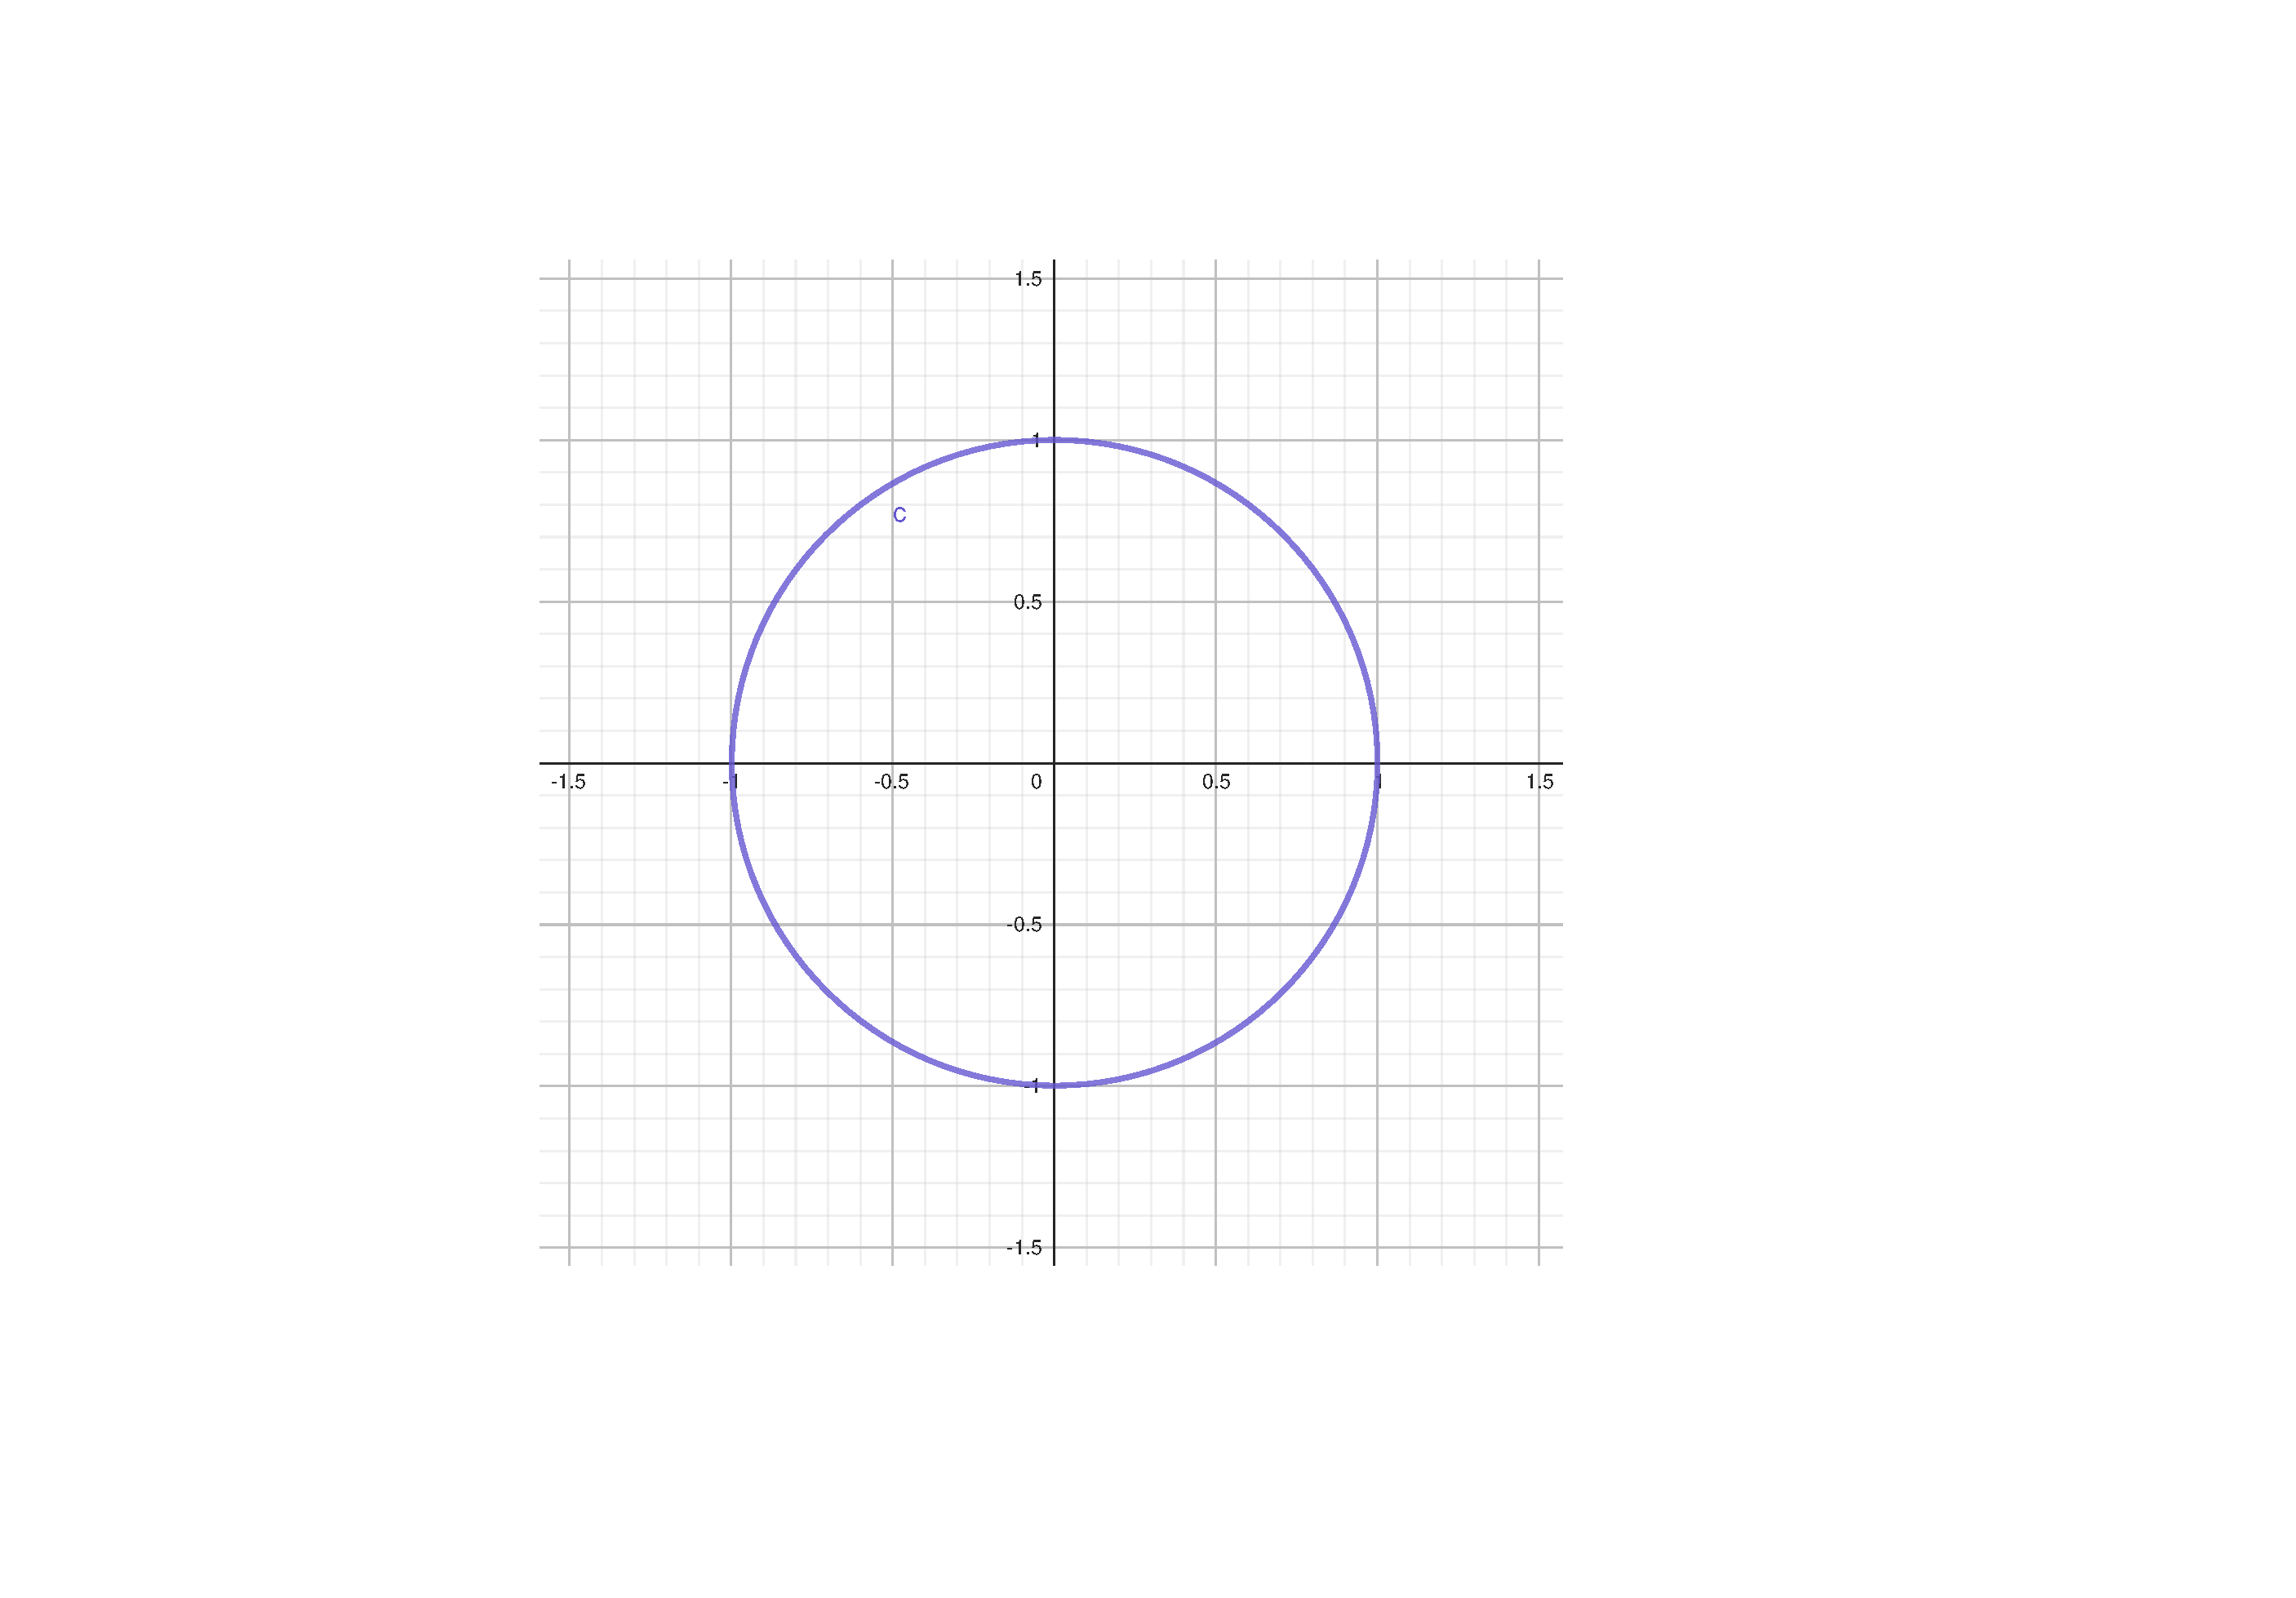
\includegraphics[width=.6\textwidth]{img/circonferenza.pdf}
	\end{figure}
	
	\noindent
	Chiamando con $C = \left(x_{C}, y_{C}\right)$ le coordinate del centro della circonferenza e con $r$ il raggio, la sua equazione generale è espressa nel seguente modo:
	\begin{equation*}
		\left(x-x_{C}\right)^{2} + \left(y-y_{C}\right)^{2} = r^{2}
	\end{equation*}
	Nel caso in cui la circonferenza fosse centrata nell'origine degli assi, ovvero $C = \left(0,0\right)$, allora l'equazione generale sarebbe ridotta a:
	\begin{equation*}
		x^{2} + y^{2} = r^{2}
	\end{equation*}
	Per essere più precisi, l'\textbf{equazione canonica} corrispondente alla circonferenza è la seguente:
	\begin{equation*}
		x^{2} + y^{2} + \alpha x + \beta y + \gamma = 0
	\end{equation*}
	Le formule più importanti per ricavare il centro della circonferenza $C$ e il raggio $r$:
	\begin{equation*}
		C = \left(-\dfrac{\alpha}{2}, -\dfrac{\beta}{2}\right) \hspace{1em} ; \hspace{1em} r = \sqrt{\dfrac{\alpha^{2}}{4} + \dfrac{\beta^{2}}{4} - \gamma}
	\end{equation*}
	Per ottenere l'equazione generale partendo dall'equazione canonica, si utilizza il metodo dei completamento dei quadrati (paragrafo~\ref{subsubsection: completamento dei quadrati}).\newline
	
	\noindent
	Per ottenere il raggio nel caso in cui sia noto il centro $C$ e un punto $P = \left(x_{P}, y_{P}\right)$ appartenente alla circonferenza, si utilizza la seguente formula:
	\begin{equation*}
		r = \sqrt{\left(x_{P} - x_{C}\right)^{2} + \left(y_{P} - y_{C}\right)^{2}}
	\end{equation*}
	Per altri approfondimenti: \href{https://www.youmath.it/formulari/formulari-di-geometria-analitica/440-circonferenza-e-cerchio-nel-piano-cartesiano.html}{YouMath}.\newpage
	
	%%%%%%%%%%%
	% Ellisse %
	%%%%%%%%%%%
	\subsubsection{Ellisse}\label{subsubsection: ellisse}
	
	Non esiste un'unica rappresentazione dell'ellisse, ma solitamente può essere facilmente riconoscibile perché di forma allungata:
	\begin{figure}[!htp]
		\centering
		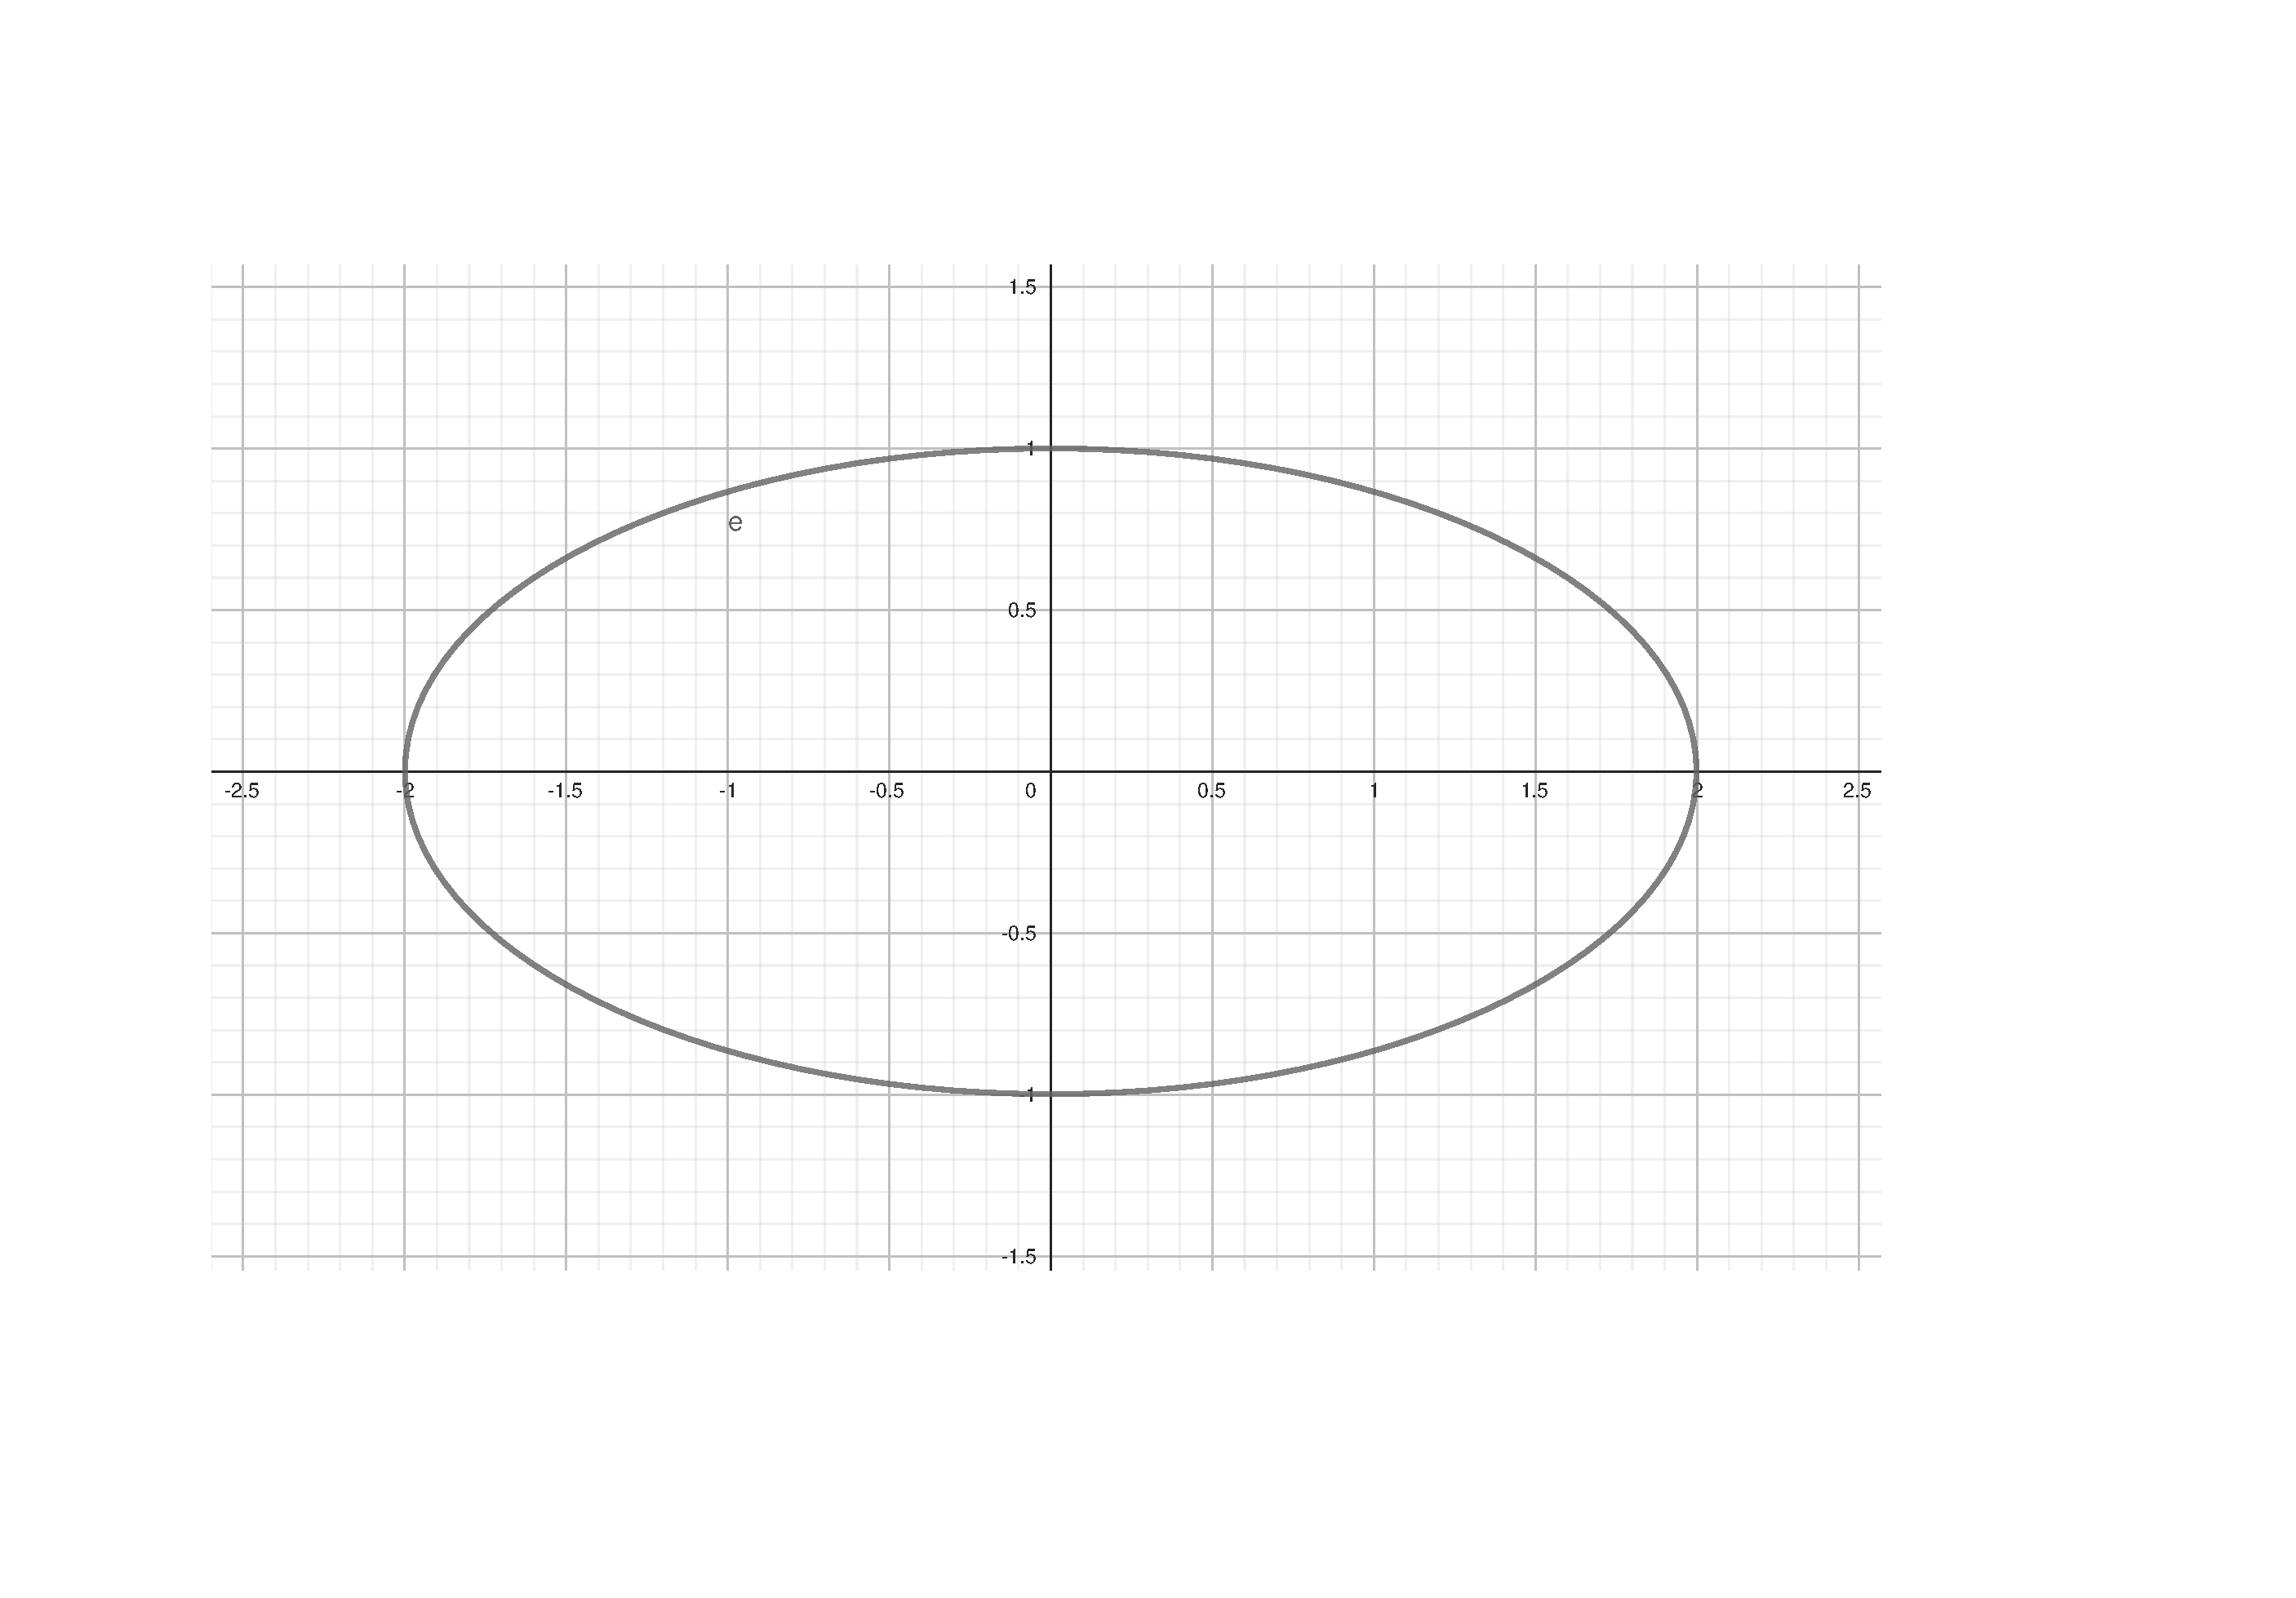
\includegraphics[width=.6\textwidth]{img/ellisse.pdf}
	\end{figure}
	
	\noindent
	Attenzione, che data l'\textbf{equazione canonica} dell'ellisse \textbf{centrata nell'origine}:
	\begin{equation*}
		\dfrac{x^{2}}{a^{2}} + \dfrac{y^{2}}{b^{2}} = 1 \hspace{2em} a \ne 0, \:\: b \ne 0
	\end{equation*}
	Il grafico corrisponde esattamente ad una circonferenza.\newline
	
	\noindent
	Un'ellisse presenta quattro vertici nel caso in cui abbia centro nell'origine. Le relative coordinate sono:
	\begin{equation*}
		V_{1,2} = \left(\pm a, 0\right) \hspace{1em} V_{3,4} = \left(0, \pm b\right)
	\end{equation*}
	Per calcolare l'eccentricità di un'ellisse (\dquotes{quanto l'ellisse è schiacciata}) si devono confrontare i due valori $a^{2}$ e $b^{2}$:
	\begin{equation*}
		\begin{array}{rclcl}
			e = \dfrac{c}{a} & \text{se} & a^{2} > b^{2} & \text{e quindi} & c = \sqrt{a^{2} - b^{2}}\\ [1em]
			e = \dfrac{c}{b} & \text{se} & b^{2} > a^{2} & \text{e quindi} & c = \sqrt{b^{2} - a^{2}}
		\end{array}
	\end{equation*}
	Il valore è compreso tra: $0 \le e < 1$.\newline
	
	\noindent
	Nel caso in cui non fosse centrata nell'origine, l'\textbf{equazione canonica} di un'\textbf{ellisse traslata}, con $C=\left(x_{C}, y_{C}\right)$ come coordinate del centro:
	\begin{equation*}
		\dfrac{\left(x-x_{C}\right)^{2}}{a^{2}} + \dfrac{\left(y-y_{C}\right)^{2}}{b^{2}} = 1
	\end{equation*}
	I relativi vertici hanno le seguenti coordinate:
	\begin{equation*}
		\begin{array}{lcl}
			V_{1} = \left(x_{C}-a, y_{C}\right) &;& V_{2} = \left(x_{C}+a, y_{C}\right) \\
			V_{3} = \left(x_{C}, y_{C}-b\right) &;& V_{4} = \left(x_{C}, y_{C}+b\right) \\
		\end{array}
	\end{equation*}
	L'\textbf{importanza dei vertici} è dovuta al fatto che se fosse necessario rappresentare l'ellisse su un piano cartesiano, grazie alle precedenti formule. È possibile ricordarsi facilmente le formule ricordando che le coordinate dei vertici sono ottenute eseguendo la somma/differenza prima sulla coordinata $x$ e poi sulla coordinata $y$.\newline
	
	\noindent
	Per altri approfondimenti: \href{https://www.youmath.it/formulari/formulari-di-geometria-analitica/445-ellisse-nel-piano-cartesiano.html}{YouMath}.\newpage

	%%%%%%%%%%%%
	% Iperbole %
	%%%%%%%%%%%%
	\subsubsection{Iperbole}\label{subsubsection: iperbole}

	Un iperbole con centro nell'origine ha un'equazione del tipo:
	\begin{equation*}
		\dfrac{x^{2}}{a^{2}} - \dfrac{y^{2}}{b^{2}} = \pm 1 \hspace{1.5em} \text{con } a \ne 0, \: b \ne 0
	\end{equation*}
	Il segno $+$ accanto all'$1$ rappresenta l'intersezione con l'asse delle ascisse ($x$), mentre il segno $-$ rappresenta l'intersezione con l'asse delle ordinate ($y$). Graficamente viene rappresentata nel seguente modo:\newline

	\begin{minipage}{.6\textwidth}
		\centering
		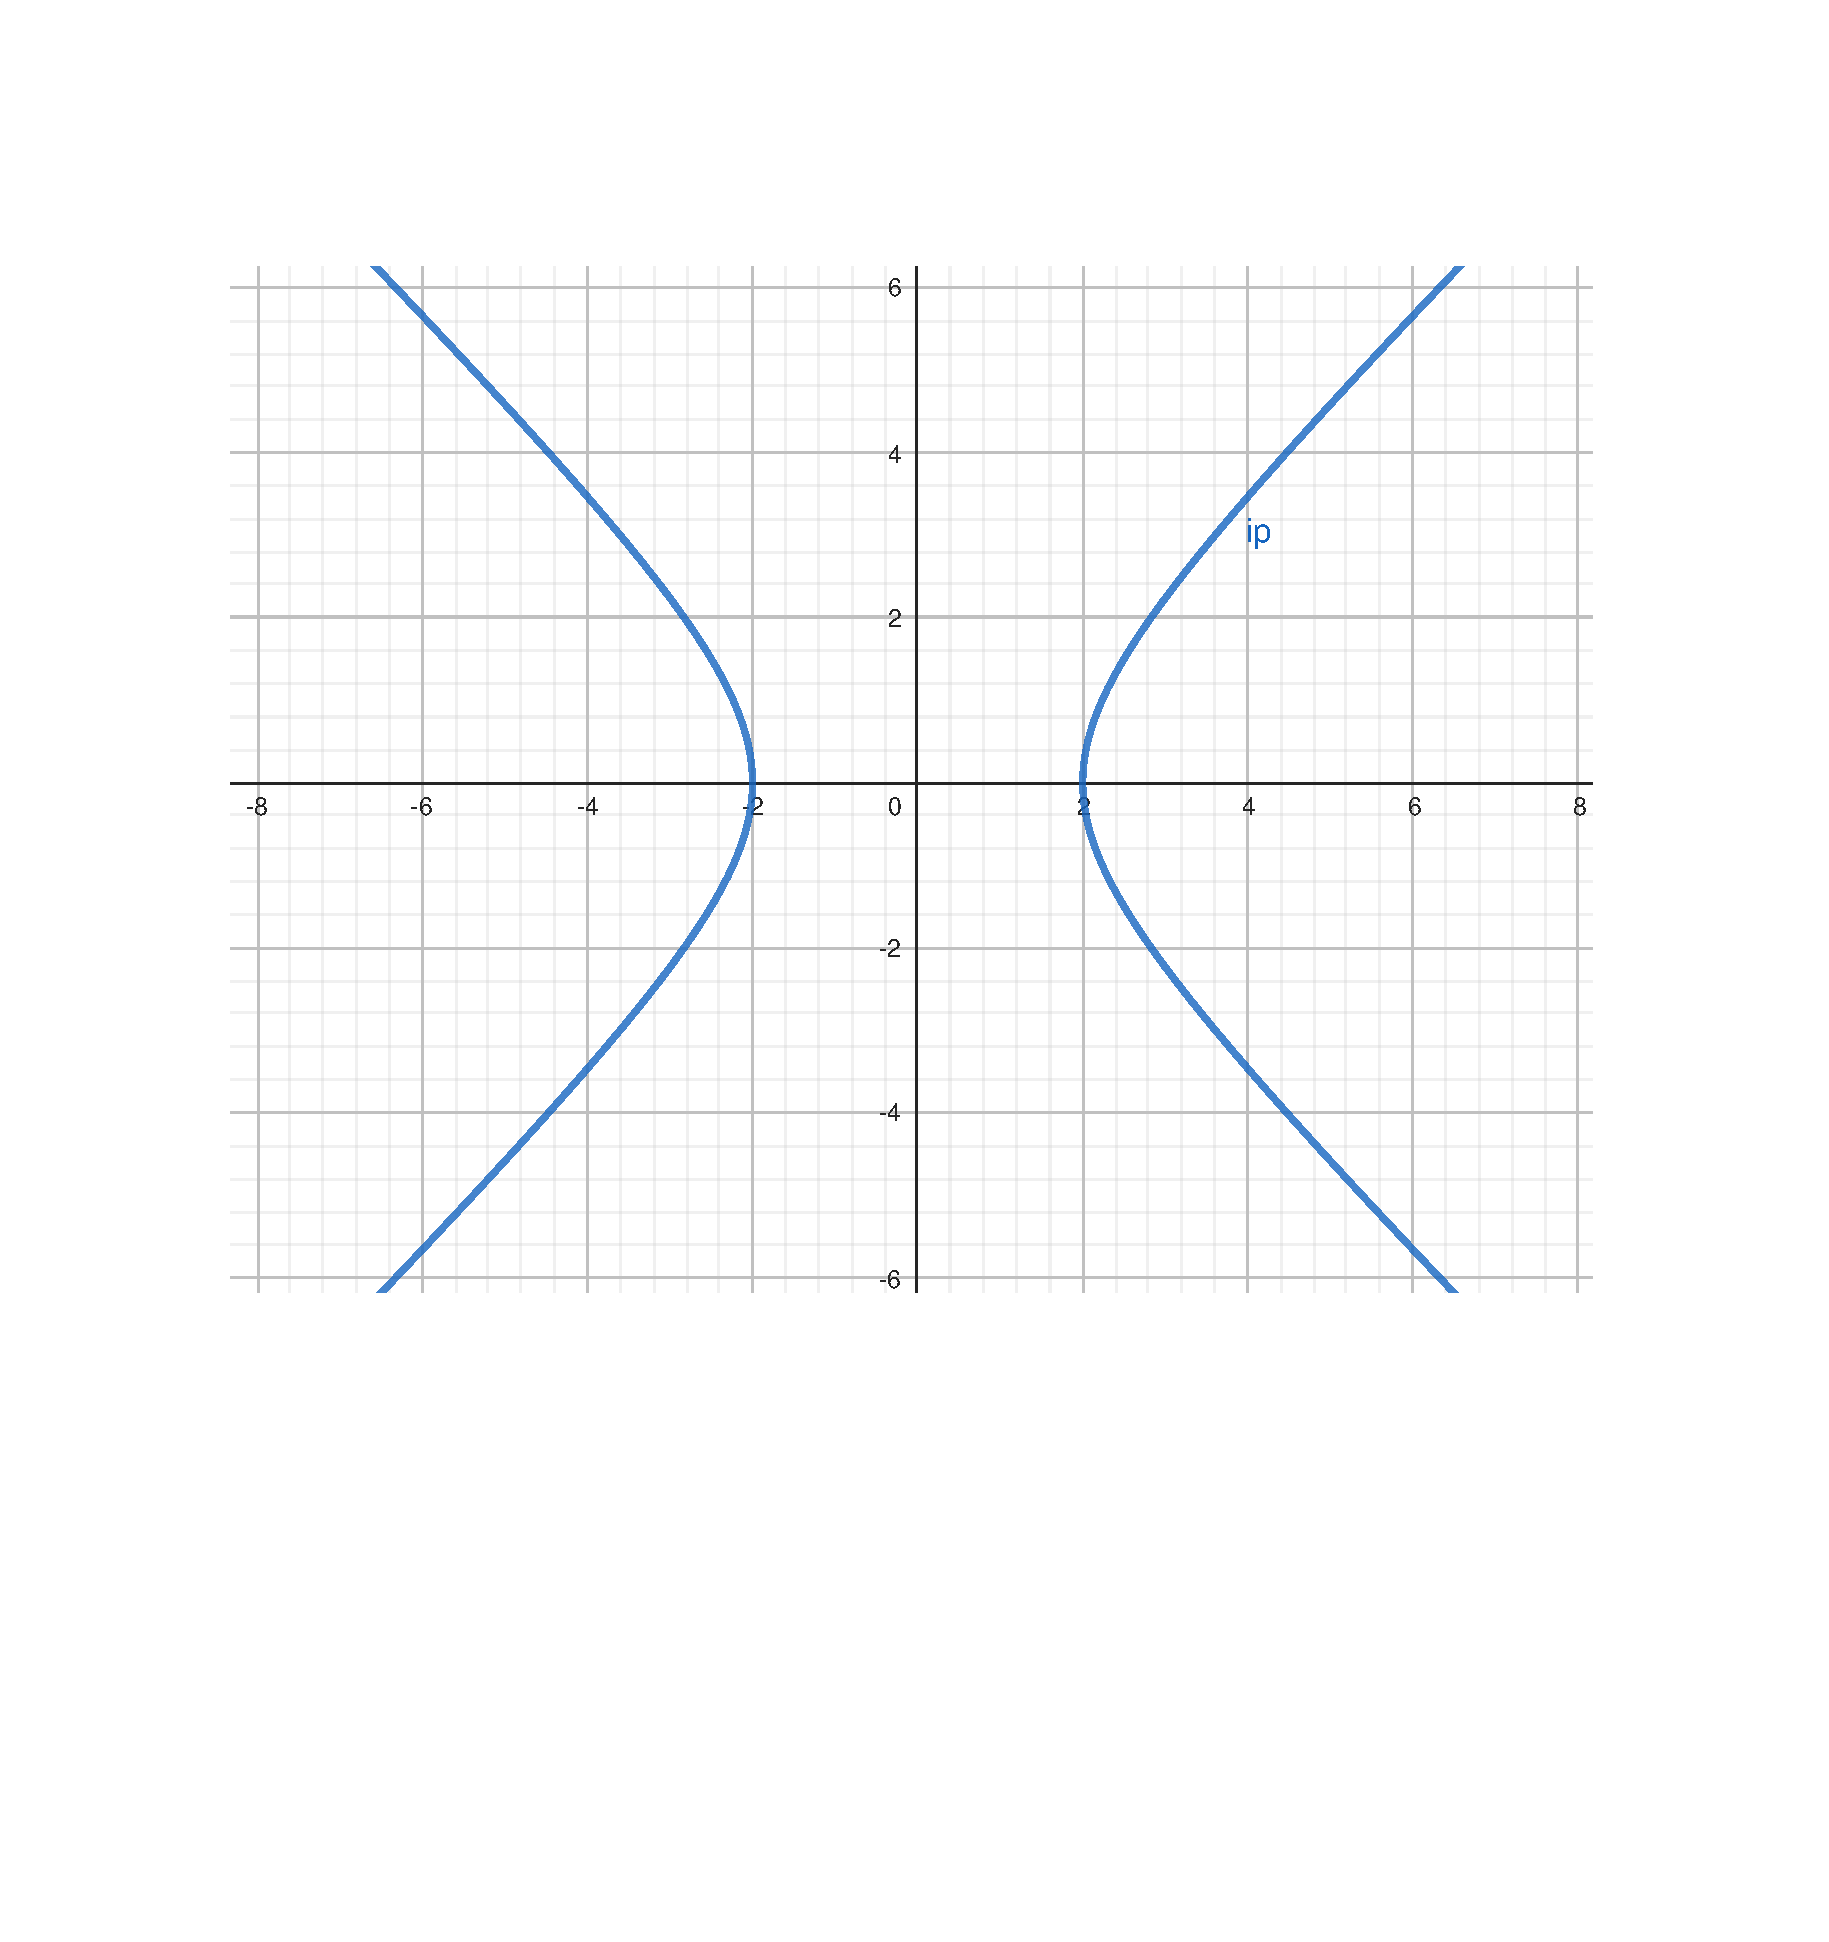
\includegraphics[width=\textwidth]{img/iperbole_ascisse.pdf}
		
		\noindent
		Con $+1$.
	\end{minipage}
	\begin{minipage}{.4\textwidth}
		\centering
		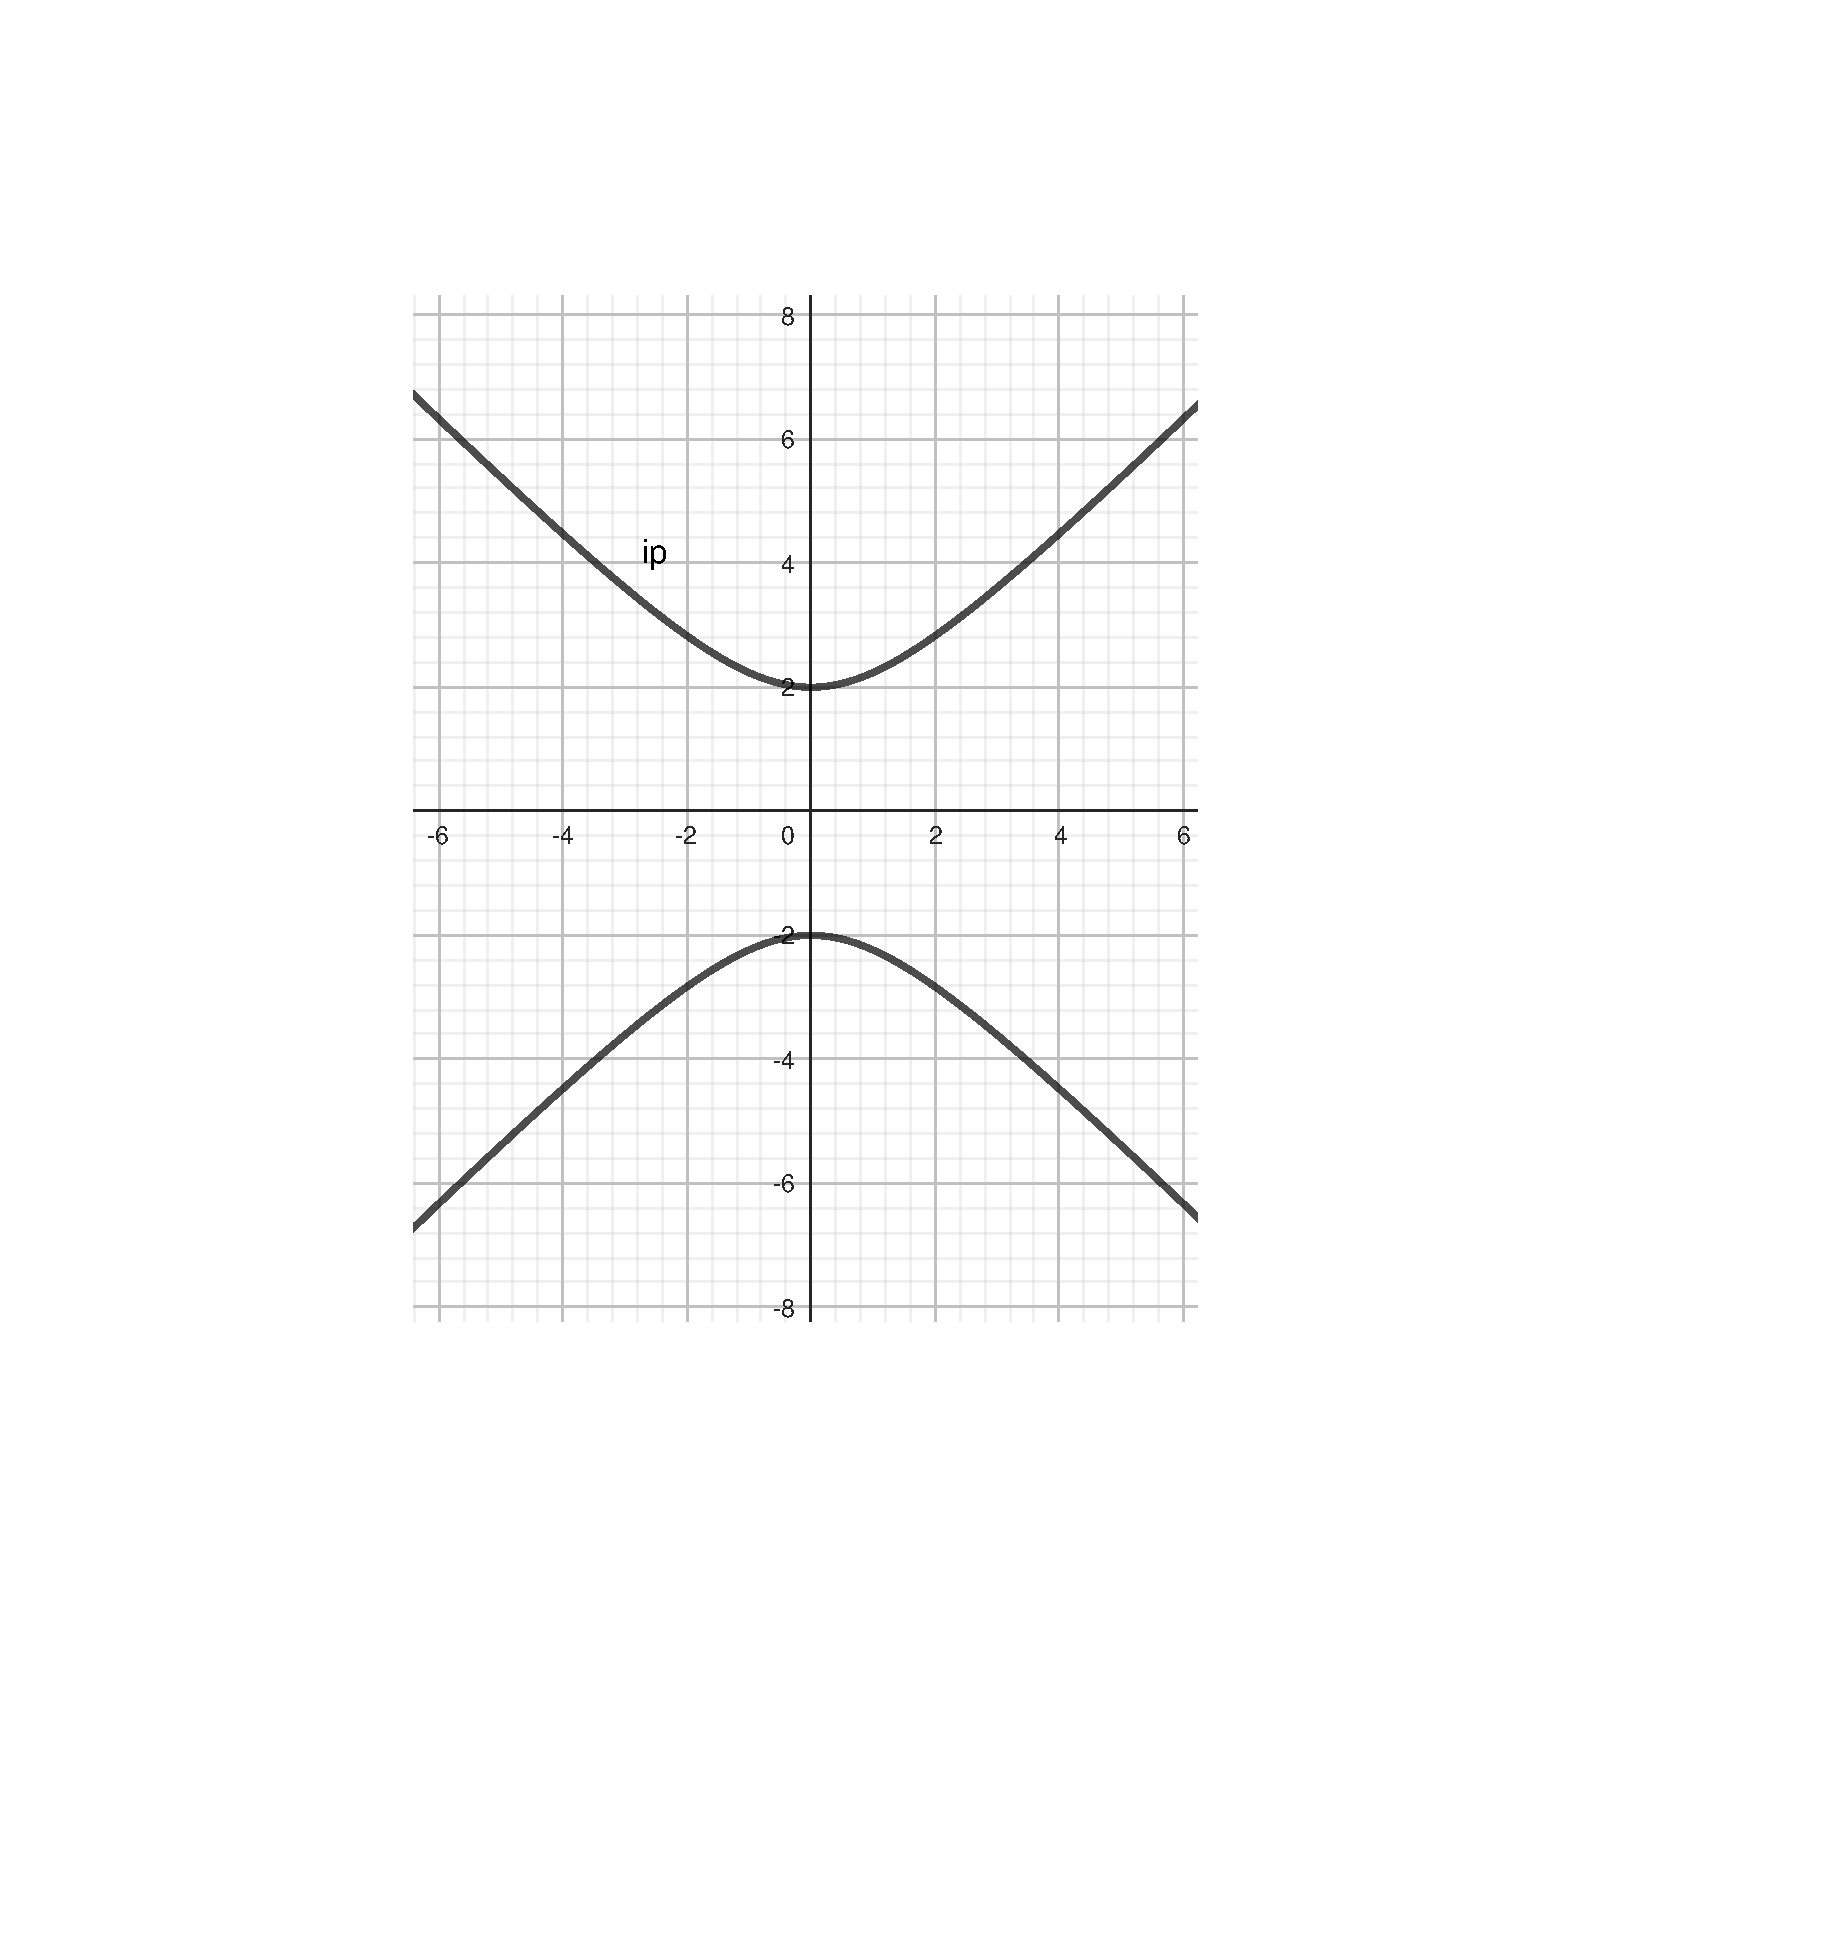
\includegraphics[width=.9\textwidth]{img/iperbole_ordinate.pdf}
		
		\noindent
		Con $-1$.
	\end{minipage}\newline

	\noindent
	Nel caso di una iperbole con gli assi paralleli agli assi cartesiani e quindi con centro in un punto $C = \left(x_{C}, y_{C}\right)$, essa è data da:
	\begin{equation*}
		\dfrac{\left(x-x_{C}\right)^{2}}{a^{2}} - \dfrac{\left(y-y_{C}\right)^{2}}{b^{2}} = \pm 1 \hspace{1.5em} \text{con } a \ne 0, \: b \ne 0
	\end{equation*}
	Dove il segno $\pm$ accanto all'$1$ indica la stessa cosa detta in precedenza.\newline
	
	\noindent
	Per altri approfondimenti: \href{https://www.youmath.it/domande-a-risposte/view/6096-equazione-iperbole.html}{YouMath}.\newpage
	
	%%%%%%%%%%%%%%%%%%%%%%%%%%%%%%
	% Completamento dei quadrati %
	%%%%%%%%%%%%%%%%%%%%%%%%%%%%%%
	\subsubsection{Completamento dei quadrati}\label{subsubsection: completamento dei quadrati}
	
	Il completamento dei quadrati è un'operazione molto potente che può essere applicata sempre (a discapito dello studente se ha senso o no applicarla!). In questo caso viene applicata ad un'ellisse.\newline
	
	\noindent
	Innanzitutto, la \textbf{prima operazione} dell'applicazione del completamento dei quadrati è il raggruppamento dei valori simili, ovverosia:
	\begin{equation*}
		\begin{array}{rcl}
			9x^{2} + 4y^{2} + 36x - 24y + 36 &=& 0 \\
			\left(9x^{2} + 36x\right) + \left(4y^{2} - 24y\right) + 36 &=& 0
		\end{array}
	\end{equation*}
	La \textbf{seconda operazione} è prendere in considerazione i termini con le $x$, e poi quelli con le $y$, e cercare un quadrato. Ovvero sia un valore $c$ tale per cui il $\Delta$ (nella formula del calcolo di un'equazione di secondo grado $\Delta = b^{2} - 4 \cdot a \cdot c$) sia uguale a zero:
	\begin{equation*}
		\begin{array}{rcl}
			9x^{2} + 36x &\longrightarrow& 36^{2} - 4 \cdot 9 \cdot c = 0 \\
			&& 36^{2} - 36c = 0 \\
			&& c = 36 \\ [1em]
			4y^{2} - 24y &\longrightarrow& 24^{2} - 4 \cdot 4 \cdot c = 0 \\
			&& 24^{2} - 16c = 0 \\
			&& c = 36
		\end{array}
	\end{equation*}
	\underline{Suggerimento}: per trovare tale valore, basta risolvere la banale equazione $b^{2} - 4 \cdot a \cdot c = 0$ con $c$ incognita e $a,b$ termini noti.\newline
	
	\noindent
	La \textbf{terza operazione} è riscrivere l'equazione con i nuovi valori $c$, ma per lasciare invariata l'equazione è necessario annullarli, ovvero scrivere $c-c$ (nessun problema, con manipolazioni algebriche si riuscirà ad evitare di ritornare al punto di inizio):
	\begin{equation*}
		\left(9x^{2} + 36x + 36 - 36\right) + \left(4y^{2} - 24y + 36 - 36\right) + 36 = 0
	\end{equation*}
	Le manipolazioni algebriche riguardano $9x^{2} + 36x + 36$ e $4y^{2} - 24y + 36$. Ovvero, si riscrivono le due espressioni come quadrati!
	\begin{equation*}
		\begin{array}{rcl}
			9x^{2} + 36x + 36 &\longrightarrow& 9\left(x+2\right)^{2} \\
			4y^{2} - 24y + 36 &\longrightarrow& 4\left(y-3\right)^{2} \\
		\end{array}
	\end{equation*}
	E si riscrive l'equazione generale:
	\begin{equation*}
		9\left(x+2\right)^{2} - 36 + 4\left(y-3\right)^{2} - 36 + 36 = 0
	\end{equation*}
	Banali semplificazioni algebriche:
	\begin{equation*}
		\begin{array}{rcl}
			9\left(x+2\right)^{2} \cancel{- 36} + 4\left(y-3\right)^{2} - 36 \cancel{+ 36} &=& 0 \\ [1em]
			\dfrac{1}{36} \cdot \cancel{9}\left(x+2\right)^{2} + \cancel{4}\left(y-3\right)^{2} &=& \cancel{36} \cdot \dfrac{1}{\cancel{36}}  \\ [1em]
			\dfrac{\left(x+2\right)^{2}}{4} + \dfrac{\left(y-3\right)^{2}}{9} &=& 1
		\end{array}
	\end{equation*}
	Quest'ultima equazione corrisponde all'equazione canonica dell'ellisse.\newpage

	%%%%%%%%%%%%
	% Esercizi %
	%%%%%%%%%%%%
	\subsubsection{Esercizi}\label{subsubsection: esercizi (geometria analitica)}
	
	Si rappresenti analiticamente le seguenti equazioni canoniche:
	\begin{enumerate}
		\item $x^{2} + y^{2} - 4x + 2y - 6 = 0$
		
		\item $x^{2} + 4y^{2} - 1 = 0$
		
		\item $x^{2} - 4y^{2} - 1 = 0$
		
		\item $x^{2} - y^{2} + x + 4y - 4 = 0$
		
		\item $2x^{2} + y^{2} + 4x - y = 0$
	\end{enumerate}
	
	\begin{flushleft}
		\example{\underline{Esercizio 1}}
	\end{flushleft}
	
	\noindent
	Data l'equazione:
	\begin{equation*}
		x^{2} + y^{2} - 4x + 2y - 6 = 0
	\end{equation*}
	Prima di rappresentare analiticamente l'equazione, è necessario guardare immediatamente i termini $x^{2}$ e $y^{2}$ per vedere se si è di fronte ad una circonferenza. Infatti, ricordando l'equazione canonica della circonferenza (pagina~\pageref{subsubsection: circonferenza}):
	\begin{equation*}
		x^{2} + y^{2} + \alpha x + \beta y + \gamma = 0
	\end{equation*}
	Si può notare una grande assomiglianza. Quindi, si procede con il calcolo delle coordinate del centro della circonferenza:
	\begin{equation*}
		C = \left(-\dfrac{\alpha}{2}, -\dfrac{\beta}{2}\right) = \left(-\dfrac{\left(-4\right)}{2}, -\dfrac{2}{2}\right) = \left(2, -1\right)
	\end{equation*}
	Si procede con il calcolo del raggio:
	\begin{equation*}
		r = \sqrt{\dfrac{\alpha^{2}}{4} + \dfrac{\beta^{2}}{4} - \gamma} = \sqrt{\dfrac{\left(-4\right)^{2}}{4} + \dfrac{\left(2\right)^{2}}{4} - \left(-6\right)} = \sqrt{4 + 1 + 6} = \sqrt{11}
	\end{equation*}
	Infine, si scrive l'equazione canonica sostituendo i valori trovati:
	\begin{equation*}
		\begin{array}{rcl}
			\left(x-x_{C}\right)^{2} + \left(y-y_{C}\right)^{2} &=& r^{2} \\ [1em]
			\left(x-2\right)^{2} + \left(y+1\right)^{2} &=& 11
		\end{array}
	\end{equation*}
	
	\begin{flushleft}
		\example{\underline{Esercizio 2}}
	\end{flushleft}
	
	\noindent
	Data l'equazione:
	\begin{equation*}
		x^{2} + 4y^{2} - 1 = 0
	\end{equation*}
	Con una piccola manipolazione algebrica si può subito vedere che si è di fronte ad un'ellisse centrata nell'origine:
	\begin{equation*}
		x^{2} + 4y^{2} = 1
	\end{equation*}
	Si procede con un po' di intuito così da ricavare la forma canonica:
	\begin{equation*}
		\dfrac{\left(x-0\right)^{2}}{1^{2}} + \dfrac{\left(y-0\right)^{2}}{\left(\frac{1}{2}\right)^{2}} = 1
	\end{equation*}
	E il risultato (forma canonica) eliminando i termini inutili:
	\begin{equation*}
		\dfrac{x^{2}}{1^{2}} + \dfrac{y^{2}}{\frac{1}{4}} = 1 \hspace{1em} \xrightarrow{\text{equivale a}} \hspace{1em} x^{2} + 4y^{2} = 1
	\end{equation*}\newpage
	
	\begin{flushleft}
		\example{\underline{Esercizio 3}}
	\end{flushleft}
	
	\noindent
	Data l'equazione:
	\begin{equation*}
		x^{2} - 4y^{2} - 1 = 0
	\end{equation*}
	Con una piccola manipolazione algebrica si ottiene l'equazione:
	\begin{equation*}
		x^{2} - 4y^{2} = 1
	\end{equation*}
	Si tratta di un'iperbole che interseca l'asse delle ascisse ($x$) perché il segno dell'$1$ è $+$ ed è centrata nell'origine perché $x$ e $y$ \dquotes{non esistono}. Quindi:
	\begin{equation*}
		\dfrac{x^{2}}{1} - \dfrac{y^{2}}{\dfrac{1}{4}} = 1
	\end{equation*}
	
	\begin{flushleft}
		\example{\underline{Esercizio 4}}
	\end{flushleft}

	\noindent
	Data l'equazione:
	\begin{equation*}
		x^{2} - y^{2} + x + 4y - 4 = 0
	\end{equation*}
	Ci si accorge immediatamente che è un iperbole a causa dei segni $x^{2}$ e $y^{2}$ discordi. Eseguendo alcune operazioni algebriche:
	\begin{equation*}
		\begin{array}{rcl}
			x^{2} - y^{2} + x + 4y - 4 &=& 0 \\ [.5em]
			x^{2} - y^{2} + x + 4y &=& 4 \\ [.5em]
			\left(x^{2}+x\right) - \left(y^{2} - 4y\right) &=& 4
		\end{array}
	\end{equation*}
	Si utilizza il completamento dei quadrati per ottenere la forma canonica:
	\begin{gather*}
		\begin{array}{rcl}
			x^{2}+x & \longrightarrow 	& 1^{2} - 4 \cdot 1 \cdot c = 0 \\ [.5em]
					&					& c = \dfrac{1}{4} \\ [1em]
			y^{2}-4y& \longrightarrow	& \left(-4\right)^{2} - 4 \cdot 1 \cdot c = 0 \\ [.5em]
					&					& c = 4
		\end{array} \\
		\begin{array}{rcl}
			\left(x^{2} + x + \dfrac{1}{4} - \dfrac{1}{4}\right) - \left(y^{2} - 4y + 4 - 4\right) &=& 4 \\ [1em]
			%
			\left[\left(x+\dfrac{1}{2}\right)^{2} - \dfrac{1}{4}\right] - \left[\left(y-2\right)^{2} - 4\right] &=& 4 \\ [1em]
			%
			\left(x+\dfrac{1}{2}\right)^{2} - \dfrac{1}{4} - \left(y-2\right)^{2} + 4 &=& 4 \\ [1em]
			%
			\left(x+\dfrac{1}{2}\right)^{2} - \left(y-2\right)^{2} &=& 4 - 4 + \dfrac{1}{4} \\ [1em]
			%
			\left(x+\dfrac{1}{2}\right)^{2} - \left(y-2\right)^{2} &=& \dfrac{1}{4} \\ [1em]
			%
			4\left(x+\dfrac{1}{2}\right)^{2} - 4\left(y-2\right)^{2} &=& 1 \\ [1em]
			%
			\dfrac{\left(x+\dfrac{1}{2}\right)^{2}}{\dfrac{1}{4}} - \dfrac{\left(y-2\right)^{2}}{\dfrac{1}{4}} &=& 1
		\end{array}
	\end{gather*}

	\newpage
	\begin{flushleft}
		\example{\underline{Esercizio 5}}
	\end{flushleft}

	\noindent
	Data l'equazione:
	\begin{equation*}
		2x^{2} + y^{2} + 4x - y = 0
	\end{equation*}
	Si utilizza il completamento dei quadrati:
	\begin{equation*}
		\begin{array}{rcl}
			2x^{2} + y^{2} + 4x - y &=& 0 \\ [.5em]
			\left(2x^{2} + 4x\right) + \left(y^{2} - y\right) &=& 0
		\end{array}
	\end{equation*}
	\begin{gather*}
		\begin{array}{rcl}
			2x^{2} + 4x & \longrightarrow 	& 4^{2} - 4 \cdot 2 \cdot c = 0 \\ [.5em]
						&					& c = 2 \\ [1em]
			y^{2}-y 	& \longrightarrow	& \left(-1\right)^{2} - 4 \cdot 1 \cdot c = 0 \\ [.5em]
						&					& c = \dfrac{1}{4}
		\end{array} \\ \\
		\begin{array}{rcl}
			\left(2x^{2} + 4x + 2 - 2\right) + \left(y^{2} - y + \dfrac{1}{4} - \dfrac{1}{4}\right) &=& 0 \\ [1em]
			%
			\left[2\left(x+1\right)^{2} - 2\right] + \left[\left(y-\dfrac{1}{2}\right)^{2} - \dfrac{1}{4}\right] &=& 0 \\ [1em]
			%
			2\left(x+1\right)^{2} - 2 + \left(y-\dfrac{1}{2}\right)^{2} - \dfrac{1}{4} &=& 0 \\ [1em]
			%
			2\left(x+1\right)^{2} + \left(y-\dfrac{1}{2}\right)^{2} &=& 2 + \dfrac{1}{4} \\ [1em]
			%
			2\left(x+1\right)^{2} + \left(y-\dfrac{1}{2}\right)^{2} &=& \dfrac{9}{4} \\ [1em]
			%
			\dfrac{4}{9} \cdot 2 \cdot \left(x+1\right)^{2} + \dfrac{4}{9} \cdot \left(y-\dfrac{1}{2}\right)^{2} &=& 1 \\ [1em]
			%
			\dfrac{\left(x+1\right)^{2}}{\dfrac{9}{8}} + \dfrac{\left(y-\dfrac{1}{2}\right)^{2}}{\dfrac{9}{4}} &=& 1 \\ [1em]
		\end{array}
	\end{gather*}
	L'equazione canonica si tratta di un'ellisse.\newpage

	%%%%%%%%%%%
	% Algebra %
	%%%%%%%%%%%
	\subsection{Algebra}\label{subsection: algebra}

	%%%%%%%%%%%%
	% Esercizi %
	%%%%%%%%%%%%
	\subsubsection{Esercizi}\label{subsubsection: esercizi (algebra)}

	Risolvere le seguenti equazioni e i seguenti sistemi di equazioni algebriche:
	\begin{enumerate}
		\item $\begin{cases}
			3x^{2}y - 6xy = 0 \\
			x^{3} + 4y^{3} - 3x^{2} = 0
		\end{cases}$

		\item $\begin{cases}
			x^{2} = \lambda x \\
			y^{2} = 4\lambda y \\
			x^{2} + 2y^{2} = 1
		\end{cases}$

		\item $\dfrac{y}{y+2} = mx^{2}$ (risolvere rispetto a $y$)
		
		\item $\dfrac{1}{y+1} = \sqrt{x+2}-1$ (risolvere rispetto a $y$)
		
		\item $\log{\dfrac{2-y}{1-y}} = x+3$ (risolvere rispetto a $y$)
	\end{enumerate}

	\begin{flushleft}
		\example{\underline{Esercizio 1}}
	\end{flushleft}
	
	\noindent
	Dato il sistema:
	\begin{equation*}
		\begin{cases}
			3x^{2}y - 6xy = 0 \\
			x^{3} + 4y^{3} - 3x^{2} = 0
		\end{cases}
	\end{equation*}
	Per trovare tutti i valori che annullano il sistema, si inizia con qualche manipolazione algebrica:
	\begin{equation*}
		\begin{cases}
			3y \left(x^{2} - 2x\right) = 0 \\
			x^{3} + 4y^{3} - 3x^{2} = 0
		\end{cases}
	\end{equation*}
	Quale valore annulla $x^{2}-2x$? Si calcola:
	\begin{equation*}
		x^{2}-2x \longrightarrow x\left(x-2\right)
	\end{equation*}
	Quindi le soluzioni sono $0$ e $2$. Per cui i valori che annullano il sistema per adesso sono:
	\begin{equation*}
		y=0 
		\longrightarrow
		\begin{cases}
			0 = 0 \\
			x^{3} - 3x^{2} = 0
		\end{cases}
		\longrightarrow
		\begin{cases}
			0 = 0 \\
			x^{2}\left(x - 3\right) = 0
		\end{cases}
		\longrightarrow
		x = 0; x = 3
	\end{equation*}
	Con $x = 0$ si è già trovata una soluzione ($y=0$), quindi si prova $x=2$:
	\begin{equation*}
		x = 2
		\longrightarrow
		\begin{cases}
			0 = 0 \\
			2^{3} + 4y^{3} - 3 \cdot 2^{2} = 0
		\end{cases}
		\longrightarrow
		\begin{cases}
			0 = 0 \\
			y^{3} = 1
		\end{cases}
	\end{equation*}
	Le soluzioni sono terminate, quindi i possibili valori sono:
	\begin{itemize}
		\item $\left(x=0, y=0\right)$
		\item $\left(x=3, y=0\right)$
		\item $\left(x=2, y=1\right)$
	\end{itemize}\newpage

	\begin{flushleft}
		\example{\underline{Esercizio 2}}
	\end{flushleft}
	
	\noindent
	Dato il sistema:
	\begin{equation*}
		\begin{cases}
			x^{2} = \lambda x \\
			y^{2} = 4\lambda y \\
			x^{2} + 2y^{2} = 1
		\end{cases}
	\end{equation*}
	Si eseguono alcune manipolazioni algebriche:
	\begin{equation*}
		\begin{cases}
			x^{2} - \lambda x = 0 \\
			y^{2} - 4\lambda y= 0 \\
			x^{2} + 2y^{2} = 1
		\end{cases}
		\longrightarrow
		\begin{cases}
			x\left(x - \lambda\right) = 0 \\
			y\left(y - 4\lambda\right) = 0 \\
			x^{2} + 2y^{2} = 1
		\end{cases}
	\end{equation*}
	I primi valori che si provano sono i soliti $x = 0$ e $y = 0$. Si inizia con $x=0$:
	\begin{equation*}
		\begin{array}{lllll}
			\begin{cases}
				0 = 0 \\
				y\left(y - 4\lambda\right) = 0 \\
				0 + 2y^{2} = 1
			\end{cases}
			&\longrightarrow&
			\begin{cases}
				0 = 0 \\
				y\left(y - 4\lambda\right) = 0 \\
				y^{2} = \dfrac{1}{2}
			\end{cases}
			&\longrightarrow&
			\begin{cases}
				0 = 0 \\
				y\left(y - 4\lambda\right) = 0 \\
				y = \pm\dfrac{1}{\sqrt{2}}
			\end{cases} \\ [2.5em]
			%
			\begin{cases}
				0 = 0 \\
				\\
				\dfrac{1}{\sqrt{2}} \left(\dfrac{1}{\sqrt{2}} - 4\lambda\right) = 0 \\
				\\
				y = \dfrac{1}{\sqrt{2}}
			\end{cases}
			&\longrightarrow&
			\begin{cases}
				0 = 0 \\
				\\
				\dfrac{1}{2} - \dfrac{4\lambda}{\sqrt{2}} = 0 \\
				\\
				y = \dfrac{1}{\sqrt{2}}
			\end{cases}
			&\longrightarrow&
			\begin{cases}
				0 = 0 \\
				\\
				\dfrac{\sqrt{2}}{4} \cdot \dfrac{4\lambda}{\sqrt{2}} = \dfrac{1}{2} \cdot \dfrac{\sqrt{2}}{4} \\
				\\
				y = \dfrac{1}{\sqrt{2}}
			\end{cases} \\ [2.5em]
			%
			\begin{cases}
				0 = 0 \\
				\\
				\lambda = \pm\dfrac{\sqrt{2}}{8} \\
				\\
				y = \dfrac{1}{\sqrt{2}}
			\end{cases}
		\end{array}
	\end{equation*}
	Si prosegue con $y=0$:
	\begin{equation*}
		\begin{array}{lllll}
			\begin{cases}
				x\left(x-\lambda\right) = 0 \\
				0 = 0 \\
				x^{2} + 0 = 1
			\end{cases}
			&\longrightarrow&
			\begin{cases}
				x\left(x-\lambda\right) = 0 \\
				0 = 0 \\
				x = \pm 1
			\end{cases}
			&\longrightarrow&
			\begin{cases}
				\lambda = \pm 1 \\
				0 = 0 \\
				x = \pm 1 
			\end{cases}
		\end{array}
	\end{equation*}
	Per concludere l'esercizio, si deve riscrivere il sistema utilizzando operazioni permesse dall'algebra:
	\begin{equation*}
		\begin{cases}
			\dfrac{1}{x} \cdot x^{2} = \lambda x \cdot \dfrac{1}{x} \\
			\\
			\dfrac{1}{y} \cdot y^{2} = 4\lambda y \cdot \dfrac{1}{y} \\
			\\
			x^{2} + 2y^{2} = 1
		\end{cases}
		\longrightarrow
		\begin{cases}
			x = \lambda \\
			y = 4\lambda \\
			x^{2} + 2y^{2} = 1
		\end{cases}
		\longrightarrow
		\begin{cases}
			x = \lambda \\
			y = 4\lambda \\
			\left(\lambda\right)^{2} + 2\left(4\lambda\right)^{2} = 1
		\end{cases}
	\end{equation*}
	È evidente che con questa piccola manipolazione algebrica, i calcoli risultano più semplici. Adesso si calcola il quadrato di lambda e si trovano le sue soluzioni per concludere l'esercizio:
	\begin{equation*}
		\begin{cases}
			x = \lambda \\
			y = 4\lambda \\
			\lambda^{2} + 32\lambda^{2} = 1
		\end{cases}
		\longrightarrow
		\begin{cases}
			x = \lambda \\
			y = 4\lambda \\
			33\lambda^{2} = 1
		\end{cases}
		\longrightarrow
		\begin{cases}
			x = \lambda \\
			y = 4\lambda \\
			\lambda^{2} = \dfrac{1}{33}
		\end{cases}
		\longrightarrow
		\begin{cases}
			x = \lambda \\
			y = 4\lambda \\
			\lambda = \pm \dfrac{1}{\sqrt{33}}
		\end{cases}
	\end{equation*}
	Si sostituisce $\lambda$ all'interno di $x$ e $y$:
	\begin{equation*}
		\begin{cases}
			x = \pm \dfrac{1}{\sqrt{33}} \\
			y = \pm \dfrac{4}{\sqrt{33}} \\
			\lambda = \pm \dfrac{1}{\sqrt{33}}
		\end{cases}
	\end{equation*}
	Le soluzioni sono terminate, sono state valutate tutte le linee del sistema. Quindi, i valori possibili sono:
	\begin{itemize}
		\item $\left(x=0, y=\dfrac{1}{\sqrt{2}}, \lambda=\dfrac{\sqrt{2}}{8}\right)$

		\item $\left(x=0, y=-\dfrac{1}{\sqrt{2}}, \lambda=-\dfrac{\sqrt{2}}{8}\right)$

		\item $\left(x=1, y=0, \lambda=1\right)$

		\item $\left(x=-1, y=0, \lambda=-1\right)$

		\item $\left(x=\dfrac{1}{\sqrt{33}}, y=\dfrac{4}{\sqrt{33}}, \lambda=\dfrac{1}{\sqrt{33}}\right)$

		\item $\left(x=-\dfrac{1}{\sqrt{33}}, y=-\dfrac{4}{\sqrt{33}}, \lambda=-\dfrac{1}{\sqrt{33}}\right)$
	\end{itemize}\newpage

	\begin{flushleft}
		\example{\underline{Esercizio 3}}
	\end{flushleft}

	\noindent
	Data l'equazione:
	\begin{equation*}
		\dfrac{y}{y+2} = mx^{2}
	\end{equation*}
	Si deve risolvere rispetto a $y$:
	\begin{equation*}
		\begin{array}{rcl}
			\dfrac{y}{y+2} &=& mx^{2} \\ [1em]
			%
			\dfrac{y+2}{1} \cdot \dfrac{y}{y+2} &=& mx^{2} \cdot \dfrac{y+2}{1} \\ [1em]
			%
			y &=& mx^{2}y + 2 m x^{2} \\ [1em]
			%
			y - mx^{2}y &=& 2 m x^{2} \\ [1em]
			%
			y\left(1 - mx^{2}\right) &=& 2 m x^{2} \\ [1em]
			%
			\dfrac{1}{1 - mx^{2}} \cdot y\left(1 - mx^{2}\right) &=& 2 m x^{2} \cdot \dfrac{1}{1 - mx^{2}} \\ [1em]
			%
			y &=& \dfrac{2 m x^{2}}{1 - mx^{2}}
		\end{array}
	\end{equation*}

	\begin{flushleft}
		\example{\underline{Esercizio 4}}
	\end{flushleft}

	\noindent
	Data l'equazione:
	\begin{equation*}
		\dfrac{1}{y+1} = \sqrt{x+2}-1
	\end{equation*}
	Si deve risolvere rispetto a $y$:
	\begin{equation*}
		\begin{array}{rcl}
			\dfrac{1}{y+1} &=& \sqrt{x+2}-1 \\ [1em]
			%
			\left(y+1\right) \cdot \dfrac{1}{y+1} &=& \left(\sqrt{x+2}-1\right) \cdot \left(y+1\right) \\ [1em]
			%
			1 &=& y\sqrt{x+2} + \sqrt{x+2} -y -1 \\ [1em]
			%
			-y\sqrt{x+2} + y &=& -2 + \sqrt{x+2} \\ [1em]
			%
			y\left(-\sqrt{x+2} + 1\right) &=& \sqrt{x+2} - 2 \\ [1em]
			%
			\dfrac{1}{1 - \sqrt{x+2}} \cdot y\left(-\sqrt{x+2} + 1\right) &=& \left(\sqrt{x+2} - 2\right) \cdot \dfrac{1}{1 - \sqrt{x+2}} \\ [1em]
			%
			y &=& \dfrac{\sqrt{x+2} -2}{1-\sqrt{x+2}}
		\end{array}
	\end{equation*}\newpage

	\begin{flushleft}
		\example{\underline{Esercizio 5}}
	\end{flushleft}

	\noindent
	Data l'equazione:
	\begin{equation*}
		\log{\dfrac{2-y}{1-y}} = x+3
	\end{equation*}
	Si deve risolvere rispetto a $y$:
	\begin{equation*}
		\begin{array}{rcl}
			\log{\dfrac{2-y}{1-y}} &=& x+3 \\ [1em]
			%
			\dfrac{2-y}{1-y} &=& 10^{x+3} \\ [1em]
			%
			\left(1-y\right) \cdot \dfrac{2-y}{1-y} &=& 10^{x+3} \cdot \left(1-y\right) \\ [1em]
			%
			2-y &=& 10^{x+3} - 10^{x+3}y \\ [1em]
			%
			-y &=& 10^{x+3} - 10^{x+3}y -2 \\ [1em]
			%
			-y + 10^{x+3}y &=& 10^{x+3} - 2 \\ [1em]
			%
			y\left(-1 + 10^{x+3}\right) &=& 10^{x+3} - 2 \\ [1em]
			%
			\dfrac{1}{-1 + 10^{x+3}} \cdot y\left(-1 + 10^{x+3}\right) &=& \left(10^{x+3} - 2\right) \cdot \dfrac{1}{-1 + 10^{x+3}} \\ [1em]
			%
			y &=& \dfrac{10^{x+3} - 2}{10^{x+3} - 1}
		\end{array}
	\end{equation*}\newpage

	%%%%%%%%%%%%%%%%%%%%%%%%%%%%%%%%%%%%%
	% Calcolo differenziale e integrale %
	%%%%%%%%%%%%%%%%%%%%%%%%%%%%%%%%%%%%%
	\subsection{Calcolo differenziale e integrale}\label{subsection: calcolo differenziale e integrale}

	%%%%%%%%%%%%%%%%%%%%%%%%%%%%%%%%%%%%%%%
	% Integrali fondamentali (o notevoli) %
	%%%%%%%%%%%%%%%%%%%%%%%%%%%%%%%%%%%%%%%
	\subsubsection{Integrali fondamentali (o notevoli)}\label{subsubsection: integrali fondamentali (o notevoli)}

	Qua di seguito si presenta una lista di integrali fondamentali (o notevoli), che consentono di calcolare qualsiasi integrale basilare. Non devono essere imparati tutti a memoria poiché la maggior parte possono essere risolti ragionando:
	\begin{itemize}
		\item $\displaystyle\int x^{n} \: \mathrm{d}x = \dfrac{x^{n+1}}{n+1}+c$ \hspace{1em} con $n \ne -1$

		\item $\displaystyle\int \dfrac{1}{x^{n}} \: \mathrm{d}x = - \dfrac{1}{\left(n-1\right) \cdot x^{n-1}}$ \hspace{1em} con $n \ne 1$

		\item $\displaystyle\int \dfrac{1}{x} \: \mathrm{d}x = \ln\left(|x|\right) + c$

		\item $\displaystyle\int \sin\left(x\right) \: \mathrm{d}x = -\cos\left(x\right) + c$ \hspace{.5em} ma \hspace{.5em} $\displaystyle\int \sin\left(n \cdot x\right) \: \mathrm{d}x = -\left(n \cdot \cos\left(n \cdot x\right)\right) + c$
		
		\item $\displaystyle\int \sin^{2}\left(x\right) \: \mathrm{d}x = \int\dfrac{1-\cos\left(2x\right)}{2} \:\mathrm{d}x$

		\item $\displaystyle\int \cos\left(x\right) \: \mathrm{d}x = \sin\left(x\right) + c$ \hspace{.5em} ma \hspace{.5em} $\displaystyle\int \cos\left(n \cdot x\right) \: \mathrm{d}x = n \cdot \sin\left(n \cdot x\right) + c$
		
		\item $\displaystyle\int \cos^{2}\left(x\right) \: \mathrm{d}x = \int\dfrac{1+\cos\left(2x\right)}{2} \:\mathrm{d}x$

		\item $\displaystyle\int \dfrac{1}{\cos^{2}\left(x\right)} \: \mathrm{d}x = \tan\left(x\right) + c$

		\item $\displaystyle\int \dfrac{1}{\sin^{2}\left(x\right)} \: \mathrm{d}x = -\cot\left(x\right) + c$

		\item $\displaystyle\int e^{x} \: \mathrm{d}x = e^{x} + c$

		\item $\displaystyle\int a^{x} \: \mathrm{d}x = \dfrac{a^{x}}{\ln\left(a\right)} + c$

		\item $\displaystyle\int \sinh\left(x\right) \: \mathrm{d}x = \cosh\left(x\right) + c$

		\item $\displaystyle\int \cosh\left(x\right) \: \mathrm{d}x = \sinh\left(x\right) + c$

		\item $\displaystyle\int \dfrac{1}{1+x^{2}} \: \mathrm{d}x = \arctan\left(x\right) + c$

		\item $\displaystyle\int \dfrac{1}{\sqrt{1-x^{2}}} \: \mathrm{d}x = \arcsin\left(x\right) + c$

		\item $\displaystyle\int \dfrac{-1}{\sqrt{1-x^{2}}} \: \mathrm{d}x = \arccos\left(x\right) + c$
	\end{itemize}
	Per altri integrali, visita il sito: \href{https://www.youmath.it/lezioni/analisi-matematica/integrali/596-integrali-notevoli.html}{YouMath}.\newpage

	%%%%%%%%%%%%%%%%%%%%%%%%%%%%%%
	% Integrare per sostituzione %
	%%%%%%%%%%%%%%%%%%%%%%%%%%%%%%
	\subsubsection{Integrare per sostituzione}\label{subsubsection: integrale per sostituzione}

	Questa tecnica risolutiva è molto potente e può essere sempre applicata. Tuttavia, si tende a non utilizzarla talvolta poiché gli integrali notevoli (cap. \ref{subsubsection: integrali fondamentali (o notevoli)}) sono più immediati.\newline

	\noindent
	Il \textbf{primo passo} è prendere in considerazione l'integrale e sostituire il valore $dx$ con:
	\begin{equation*}
		dx = \dfrac{1}{t'} \: \mathrm{d}t
	\end{equation*}
	E cercare un valore $t$ comodo così da effettuare sostituzioni intelligenti. Per esempio, dato l'integrale:
	\begin{equation*}
		\displaystyle\int x^{3}e^{-x^{2}} \: \mathrm{d}x
	\end{equation*}
	Si può sostituire $dx$ scegliendo come $t$ la $x^{2}$, infatti:
	\begin{gather*}
		t = x^{2} \hspace{2em} t' = 2x \hspace{2em} dx = \dfrac{1}{2x} \: \mathrm{d}t \\ \\
		\displaystyle\int x^{3}e^{-x^{2}} \cdot \dfrac{1}{2x} \: \mathrm{d}t
		\longrightarrow
		\displaystyle\int x^{\cancelto{2}{3}}e^{-x^{2}} \cdot \dfrac{1}{2\cancel{x}} \: \mathrm{d}t
		\longrightarrow
		\displaystyle\dfrac{1}{2}\int x^{2} \cdot e^{-x^{2}} \: \mathrm{d}t
		\longrightarrow
		\displaystyle\dfrac{1}{2}\int t \cdot e^{-t} \: \mathrm{d}t
	\end{gather*}
	Una volta risolto l'integrale, si ritorna alla forma con $x$ andando a risostituire.
	
	\longline

	%%%%%%%%%%%%%%%%%%%%%%%
	% Integrare per parti %
	%%%%%%%%%%%%%%%%%%%%%%%
	\subsubsection{Integrare per parti}\label{subsubsection: integrare per parti}

	L'integrazione per parti è un metodo che viene applicato quando:
	\begin{itemize}
		\item Se l'integranda è il prodotto di due funzioni;
		\item Se l'integranda è il prodotto di due funzioni, e una di queste è la derivata di una primitiva immediata (come esponenziali, trigonometriche, potenze, etc).
	\end{itemize}
	L'applicazione è la seguente a seconda dell'integrale definito o indefinito:	
	\begin{itemize}
		\item $\displaystyle \int_{a}^{b} f\left(x\right) g'\left(x\right) \: \mathrm{d}x = f\left(b\right)g\left(b\right) - f\left(a\right)g\left(a\right) - \int_{a}^{b} f'\left(x\right)g\left(x\right) \:\mathrm{d}x$

		\item $\displaystyle \int f\left(x\right) g'\left(x\right) \: \mathrm{d}x = f\left(x\right)g\left(x\right) - \int f'\left(x\right)g\left(x\right) \: \mathrm{d}x$
	\end{itemize}
	Un esempio valido è il seguente integrale:
	\begin{equation*}
		\displaystyle \int t \cdot e^{-t} \: \mathrm{d}t
	\end{equation*}
	Si prosegue per parti:
	\begin{equation*}
		f\left(t\right) = t \hspace{2em} f'\left(t\right) = 1 \hspace{2em} g'\left(t\right) = e^{-t} \hspace{2em} g\left(t\right) = - e^{-t}
	\end{equation*}
	E si va alla sostituzione:
	\begin{equation*}
		\displaystyle \int t \cdot e^{-t} \: \mathrm{d}t = t \cdot \left(-e^{-t}\right) - \int 1 \cdot \left(-e^{-t}\right)
	\end{equation*}\newpage

	%%%%%%%%%%%%%%%%%%%%%%%%%%%%%%%%%%%%%%%
	% Decomposizione in frazioni parziali %
	%%%%%%%%%%%%%%%%%%%%%%%%%%%%%%%%%%%%%%%
	\subsubsection{Decomposizione in frazioni parziali}\label{subsubsection: decomposizione in frazioni parziali}

	La decomposizione in frazioni parziali è un metodo per trasformare il rapporto tra due polinomi in una somma di frazioni più semplici.\newline
	
	\noindent
	Questa tecnica viene inserita nel paragrafo degli integrali poiché spesso viene utilizzata per calcolare integrali che presentano frazioni apparentemente complesse.\newline

	\noindent
	Si presenta un integrale complesso:
	\begin{equation*}
		\displaystyle\int\dfrac{x^{2}}{\left(x^{2} - 1\right)^{2}} \: \mathrm{d}x
	\end{equation*}
	Innanzitutto, si eseguono alcune \textbf{operazioni preliminari}, ovverosia si prepara la frazione scomponendola il più possibile. In questo caso, al denominatore è possibile scomporre $x^{2}-1$ (ricordando $x^{2} = 1 \rightarrow x = \pm 1$):
	\begin{equation*}
		\displaystyle\int\dfrac{x^{2}}{\left[\left(x-1\right)\left(x+1\right)\right]^{2}} \: \mathrm{d}x
	\end{equation*}
	E inoltre, dato che vi è una potenza e una moltiplicazione all'interno, è possibile scomporre ancora di più:
	\begin{equation*}
		\displaystyle\int\dfrac{x^{2}}{\left(x-1\right)^{2}\left(x+1\right)^{2}} \: \mathrm{d}x
	\end{equation*}
	Adesso si parte con il vero algoritmo. Il \textbf{primo passo} è prendere ciascun fattore del denominatore e creare la sua corrispondenza con le lettere:
	\begin{equation*}
		\begin{array}{rcl}
			\left(x-1\right)^{2} &\longrightarrow& \dfrac{A}{x-1} + \dfrac{B}{\left(x-1\right)^{2}} \\ [1em]
			\left(x+1\right)^{2} &\longrightarrow& \dfrac{C}{x+1} + \dfrac{D}{\left(x-1\right)^{2}}
		\end{array}
	\end{equation*}
	Come si può notare, si parte dal grado minimo del fattore preso in considerazione, e lo si aumenta di grado fino a che non si trova il grado originario. Nel caso in cui ci fosse stato:
	\begin{equation*}
		\displaystyle \int\dfrac{1}{x\left(x-3\right)} \: \mathrm{d}x
	\end{equation*}
	Sarebbe bastato banalmente:
	\begin{equation*}
		\begin{array}{rcl}
			x &\longrightarrow& \dfrac{A}{x} \\ [1em]
			x-3 &\longrightarrow& \dfrac{B}{x-3}
		\end{array}
	\end{equation*}
	Ovviamente le lettere sono numeri reali da determinare (lo scopo dell'algoritmo). Quindi, il \textbf{secondo passo} è riscrivere i termini appena notati come un'uguaglianza:
	\begin{equation*}
		\dfrac{x^{2}}{\left(x^{2} - 1\right)^{2}} = \dfrac{A}{x-1} + \dfrac{B}{\left(x-1\right)^{2}} + \dfrac{C}{x+1} + \dfrac{D}{\left(x-1\right)^{2}}
	\end{equation*}
	Il \textbf{terzo passo} è mettere tutti i termini a denominatore comune:
	\begin{equation*}
		\dfrac{x^{2}}{\left(x^{2} - 1\right)^{2}} = \dfrac{
			A\left(x-1\right)\left(x+1\right)^{2} +
			B\left(x+1\right)^{2} +
			C\left(x-1\right)^{2}\left(x+1\right) +
			D\left(x-1\right)^{2}
		}{
			\left(x-1\right)^{2}\left(x+1\right)^{2}
		}
	\end{equation*}
	Il \textbf{quarto passo} è eliminare il denominatore:
	\begin{equation*}
		x^{2} = A\left(x-1\right)\left(x+1\right)^{2} +
		B\left(x+1\right)^{2} +
		C\left(x-1\right)^{2}\left(x+1\right) +
		D\left(x-1\right)^{2}
	\end{equation*}
	Il \textbf{quinto passo} è eseguire i calcoli e cercare di raggruppare i termini in comune:
	\begin{equation*}
		\begin{array}{rcl}
			x^{2} &=& A\left(x-1\right)\left(x+1\right)^{2} + B\left(x+1\right)^{2} + C\left(x-1\right)^{2}\left(x+1\right) + D\left(x-1\right)^{2} \\ [1em]
			%
			x^{2} &=& Ax^{3} + Cx^{3} + Ax^{2} - Cx^{2} + Dx^{2} - Ax + 2Bx - Cx - A + B + C + D \\ [1em]
			%
			x^{2} &=& \left(A+C\right)x^{3} + \left(A+B-C+D\right) x^{2} + \left(-A+2B-C-2D\right)x - A+B+C+D
		\end{array}
	\end{equation*}
	Il \textbf{sesto passo} è costruire un sistema che avrà come incognite le lettere e come valori noti $1$ se vi è una corrispondenza con le $x$, $0$ altrimenti. Quindi, in questo caso solo il fattore $\left(A+B-C+D\right)$ avrà $1$ nel sistema:
	\begin{equation*}
		\begin{cases}
			A+C = 0 \\
			A+B-C+D = 1 \\
			-A+2B-C-2D = 0 \\
			-A +B +C +D = 0
		\end{cases}
	\end{equation*}
	Usando il metodo di sostituzione si ottengono i valori:
	\begin{equation*}
		A=\dfrac{1}{4}; \hspace{.5em}
		B=\dfrac{1}{4}; \hspace{.5em}
		C=-\dfrac{1}{4}; \hspace{.5em}
		D=\dfrac{1}{4};
	\end{equation*}
	Il \textbf{settimo passo} è sostituire i valori trovati all'interno dell'uguaglianza scritta con le lettere:
	\begin{equation*}
		\begin{array}{rcl}
			\dfrac{x^{2}}{\left(x^{2} - 1\right)^{2}} &=& \dfrac{A}{x-1} + \dfrac{B}{\left(x-1\right)^{2}} + \dfrac{C}{x+1} + \dfrac{D}{\left(x-1\right)^{2}} \\ [2em]
			%
			\dfrac{x^{2}}{\left(x^{2} - 1\right)^{2}} &=& \dfrac{\dfrac{1}{4}}{x-1} + \dfrac{\dfrac{1}{4}}{\left(x-1\right)^{2}} + \dfrac{\dfrac{1}{4}}{x+1} + \dfrac{\dfrac{1}{4}}{\left(x-1\right)^{2}} \\ [2em]
			%
			\dfrac{x^{2}}{\left(x^{2} - 1\right)^{2}} &=& \dfrac{1}{4\left(x-1\right)} + \dfrac{1}{4\left(x-1\right)^{2}} + \dfrac{1}{4\left(x+1\right)} + \dfrac{1}{4\left(x+1\right)^{2}}
		\end{array}
	\end{equation*}
	L'\textbf{ottavo} e ultimo \textbf{passo} è riscrivere l'integrale con i termini appena trovati. Adesso è evidente che il calcolo risulta molto più semplice:
	\begin{equation*}
		\displaystyle\int\dfrac{x^{2}}{\left(x^{2} - 1\right)^{2}} \: \mathrm{d}x = \int \left(
			\dfrac{1}{4\left(x-1\right)} + \dfrac{1}{4\left(x-1\right)^{2}} + \dfrac{1}{4\left(x+1\right)} + \dfrac{1}{4\left(x+1\right)^{2}}
		\right) \: \mathrm{d}x
	\end{equation*}
	Fonte: \href{https://www.youmath.it/forum/sezione-speciale-per-i-topic-a-pagamento/94247-metodo-delle-frazioni-parziali-applicato-agli-integrali-indefiniti.html}{YouMath}.\newpage

	%%%%%%%%%%%%
	% Esercizi %
	%%%%%%%%%%%%
	\subsubsection{Esercizi}\label{subsubsection: esercizi (calcolo differenziale e integrale)}

	Calcolare la derivata delle seguenti funzioni:
	\begin{enumerate}
		\item $f\left(x\right) = \sqrt{\cos\left(3x+1\right)}$

		\item $f\left(x\right) = \left(2x+1\right) \exp\left(-\dfrac{1}{2}x^{2}\right)$
	\end{enumerate}
	Calcolare i seguenti integrali:
	\begin{enumerate}[resume]
		\item $\displaystyle \int\dfrac{1}{x^{2} - 3x} \: \mathrm{d}x$

		\item $\displaystyle \int x^{3} e^{-x^{2}} \: \mathrm{d}x$

		\item $\displaystyle \int\dfrac{1}{\sqrt[3]{t-1}} \: \mathrm{d}t$

		\item $\displaystyle \int\dfrac{t}{\sqrt{t^{2} - 1}} \: \mathrm{d}t$

		\item $\displaystyle \int\dfrac{1}{4 + y^{2}} \: \mathrm{d}y$

		\item $\displaystyle \int x \sqrt{1+x^{2}} \: \mathrm{d}x$
	\end{enumerate}

	\begin{flushleft}
		\example{\underline{Esercizio 1}}
	\end{flushleft}

	\noindent
	Data la funzione:
	\begin{equation*}
		f\left(x\right) = \sqrt{\cos\left(3x+1\right)}
	\end{equation*}
	La sua derivata è la seguente:
	\begin{equation*}
		\begin{array}{rcl}
			f'\left(x\right) &=& \dfrac{1}{2 \cdot \sqrt{\left(\cos\left(3x+1\right)\right)^{1}}} \cdot \left(-\sin\left(3x+1\right) \cdot 3\right) \\ [2em]
			%
			f'\left(x\right) &=& - \dfrac{3 \sin\left(3x+1\right)}{2 \sqrt{\cos\left(3x+1\right)}}
		\end{array}
	\end{equation*}

	\begin{flushleft}
		\example{\underline{Esercizio 2}}
	\end{flushleft}

	\noindent
	Data la funzione:
	\begin{equation*}
		f\left(x\right) = \left(2x+1\right) \exp\left(-\dfrac{1}{2}x^{2}\right)
	\end{equation*}
	La sua derivata è la seguente:
	\begin{equation*}
		\begin{array}{rcl}
			f'\left(x\right) &=& 2 \cdot \exp\left(-\dfrac{1}{2}x^{2}\right) + \left(2x+1\right) \cdot \left(-x\right) \cdot \exp\left(-\dfrac{1}{2}x^{2}\right)\\ [2em]
			%
			f'\left(x\right) &=& 2 \cdot \exp\left(-\dfrac{1}{2}x^{2}\right) - 2x^{2}\exp\left(-\dfrac{1}{2}x^{2}\right) - x\exp\left(-\dfrac{1}{2}x^{2}\right)
		\end{array}
	\end{equation*}\newpage

	\begin{flushleft}
		\example{\underline{Esercizio 3}}
	\end{flushleft}

	\noindent
	Dato l'integrale:
	\begin{equation*}
		\displaystyle \int\dfrac{1}{x^{2} - 3x} \: \mathrm{d}x
	\end{equation*}
	Si procede con la risoluzione:
	\begin{equation*}
		\begin{array}{rcl}
			&& \displaystyle \int\dfrac{1}{x^{2} - 3x} \: \mathrm{d}x \\ [1em]
			%
			&=& \displaystyle \int\dfrac{1}{x\left(x-3\right)} \: \mathrm{d}x \\ [2em]
			%
			&\downarrow& \text{si utilizza la decomposizione in frazioni parziali (pag. \pageref{subsubsection: decomposizione in frazioni parziali})} \\ [1.5em]
			%
			\dfrac{1}{x^{2}-3x} &=& \dfrac{A}{x} + \dfrac{B}{x-3} \\ [2em]
			%
			\dfrac{1}{x^{2}-3x} &=& \dfrac{A\left(x-3\right) + B\left(x\right)}{x\left(x-3\right)} \\ [2em]
			%
			\dfrac{1}{x^{2}-3x} &=& \dfrac{Ax - 3A + Bx}{x\left(x-3\right)} \\ [2em]
			%
			x\left(x-3\right) \cdot \dfrac{1}{x^{2}-3x} &=& \dfrac{\left(A + B\right)x - 3A}{x\left(x-3\right)} \cdot x\left(x-3\right) \\ [2em]
			%
			1 &=& \left(A + B\right)x - 3A \\ [2em]
			%
			&=& \begin{cases}
				A + B = 0 \\
				-3A = 1
			\end{cases} \longrightarrow
			\begin{cases}
				B = \frac{1}{3} \\
				A = -\frac{1}{3}
			\end{cases} \\ [2em]
			%
			\dfrac{1}{x^{2}-3x} &=& \dfrac{-\frac{1}{3}}{x} + \dfrac{\frac{1}{3}}{x-3} \\ [2em]
			%
			\dfrac{1}{x^{2}-3x} &=& -\dfrac{1}{3x} + \dfrac{1}{3\left(x-3\right)} \\ [2em]
			%
			&\downarrow& \text{si torna a risolvere l'integrale sostituendo il valore trovato} \\ [1.5em]
			%
			&=& \displaystyle\int -\dfrac{1}{3x} + \dfrac{1}{3\left(x-3\right)} \: \mathrm{d}x \\ [2em]
			%
			&=& \displaystyle-\int \dfrac{1}{3x} \: \mathrm{d}x + \displaystyle\int \dfrac{1}{3\left(x-3\right)} \: \mathrm{d}x \\ [2em]
			%
			&=& \displaystyle -\dfrac{1}{3}\int \dfrac{1}{x} \: \mathrm{d}x + \displaystyle\dfrac{1}{3}\int \dfrac{1}{x-3} \: \mathrm{d}x \\ [2em]
		\end{array}
	\end{equation*}\newpage

	\noindent
	Per risolvere questo integrale, si sfrutta uno degli integrali notevoli (pagina \pageref{subsubsection: integrali fondamentali (o notevoli)}):
	\begin{equation*}
		\begin{array}{rcl}
			&=& \displaystyle -\dfrac{1}{3}\int \dfrac{1}{x} \: \mathrm{d}x + \displaystyle\dfrac{1}{3}\int \dfrac{1}{x-3} \: \mathrm{d}x \\ [2em]
			%
			&=& -\dfrac{1}{3}\ln\left(x\right) + \dfrac{1}{3}\ln\left(x-3\right) + c \hspace{1em} c \in \mathbb{R}
		\end{array}
	\end{equation*}
	Questo è vero perché si ricorda che:
	\begin{equation*}
		f\left(x\right) = \ln\left(x-3\right) \longrightarrow f'\left(x\right) = \dfrac{1}{x-3} \cdot \dfrac{d}{dx}\left(x-3\right) = \dfrac{1}{x-3} \cdot 1
	\end{equation*}

	\longline

	\begin{flushleft}
		\example{\underline{Esercizio 4}}
	\end{flushleft}
	
	\noindent
	Dato l'integrale:
	\begin{equation*}
		\displaystyle \int x^{3} e^{-x^{2}} \: \mathrm{d}x
	\end{equation*}
	Si procede con la risoluzione usando inizialmente il metodo di sostituzione:
	\begin{equation*}
		\begin{array}{rcl}
			&& \displaystyle \int x^{3} e^{-x^{2}} \: \mathrm{d}x \\ [2em]
			%
			&\downarrow& \text{si imposta }t = x^{2}; \:\: t' = 2x; \:\: \mathrm{d}x = \dfrac{1}{t'}\:\mathrm{d}t \\ [1.5em]
			%
			&=& \displaystyle \int x^{3} e^{-x^{2}} \cdot \dfrac{1}{2x} \: \mathrm{d}t \\ [2em]
			%
			&=& \displaystyle \int x^{\cancelto{2}{3}} e^{-x^{2}} \cdot \dfrac{1}{2\cancel{x}} \: \mathrm{d}t \longrightarrow \displaystyle \int x^{2} e^{-x^{2}} \cdot \dfrac{1}{2} \: \mathrm{d}t \\ [2em]
			%
			&\downarrow& \text{si termina la sostituzione} \\ [1.5em]
			%
			&=& \displaystyle \dfrac{1}{2} \cdot \int t \cdot e^{-t} \: \mathrm{d}t \\ [2em]
			%
			&\downarrow& \text{data la moltiplicazione, adesso si cambia manovra e si utilizza il metodo per parti} \\ [1.5em]
			%
			&\downarrow& f\left(t\right) = t \hspace{2em} f'\left(t\right) = 1 \hspace{2em} g'\left(t\right) = e^{-t} \hspace{2em} g\left(t\right) = - e^{-t} \\ [2em]
			%
			&=& \dfrac{1}{2}\left[t \cdot \left(-e^{-t}\right) - \displaystyle\int 1 \cdot \left(-e^{-t}\right) \: \mathrm{d}t \right] \\ [2em]
			%
			&=& \dfrac{1}{2}\left[t \cdot \left(-e^{-t}\right) - e^{-t}\right] \\ [2em]
			%
			&\downarrow& \text{si ritorna alla }x \\ [1.5em]
			%
			&=& \dfrac{1}{2} \left(-x^{2}e^{-x^{2}} - e^{-x^{2}}\right)
			\longrightarrow
			-\dfrac{x^{2}e^{-x^{2}}}{2} - \dfrac{e^{-x^{2}}}{2}
			\longrightarrow
			-\dfrac{x^{2}+1}{2e^{x^{2}}}
		\end{array}
	\end{equation*}\newpage

	\begin{flushleft}
		\example{\underline{Esercizio 5}}
	\end{flushleft}
	
	\noindent
	Dato l'integrale:
	\begin{equation*}
		\displaystyle \int\dfrac{1}{\sqrt[3]{t-1}} \: \mathrm{d}t
	\end{equation*}
	Si inizia con il metodo di sostituzione:
	\begin{equation*}
		\begin{array}{rcl}
			&& \displaystyle \int \dfrac{1}{\sqrt[3]{t-1}} \: \mathrm{d}t \\ [2em]
			%
			&\downarrow& u = t-1; \hspace{2em} u' = 1; \hspace{2em} dt = \dfrac{1}{u'} \: \mathrm{d}u \\ [1.5em]
			%
			&=& \displaystyle \int \dfrac{1}{\sqrt[3]{u}} \cdot \dfrac{1}{1} \: \mathrm{d}u \\ [2em]
			%
			&=& \displaystyle \int \dfrac{1}{u^{\frac{1}{3}}} \: \mathrm{d}u \\ [2em]
			%
			&\downarrow& \text{si applica l'integrale notevole: }\displaystyle\int \dfrac{1}{x^{n}} \: \mathrm{d}x = - \dfrac{1}{\left(n-1\right) \cdot x^{n-1}} \\ [2em]
			%
			&=& -\dfrac{1}{\left(\dfrac{1}{3} - 1\right) \cdot u^{\frac{1}{3}-1}} \\ [3em]
			%
			&\downarrow& \text{si ritorna alla }t \\ [1.5em]
			%
			&=& - \dfrac{1}{-\dfrac{2}{3} \cdot \left(t-1\right)^{-\frac{2}{3}}} \\ [2em]
			%
			&=& - \dfrac{\sqrt[3]{\left(t-1\right)^{2}}}{-\dfrac{2}{3}} \\ [2.5em]
			%
			&=& \dfrac{3\sqrt[3]{\left(t-1\right)^{2}}}{2}
		\end{array}
	\end{equation*}\newpage

	\begin{flushleft}
		\example{\underline{Esercizio 6}}
	\end{flushleft}
	
	\noindent
	Dato l'integrale:
	\begin{equation*}
		\displaystyle \int\dfrac{t}{\sqrt{t^{2} - 1}} \: \mathrm{d}t
	\end{equation*}
	Si procede con la risoluzione:
	\begin{equation*}
		\begin{array}{rcl}
			&& \displaystyle \int\dfrac{t}{\sqrt{t^{2} - 1}} \: \mathrm{d}t \\ [2em]
			%
			&=& \displaystyle \int t \cdot \dfrac{1}{\sqrt{t^{2} - 1}} \: \mathrm{d}t \\ [2em]
			%
			&\downarrow& \text{si applica il metodo di sostituzione } u = t^{2}-1; \hspace{2em} u' = 2t; \hspace{2em} dt = \dfrac{1}{u'} \: \mathrm{d}u \\ [2em]
			%
			&=& \displaystyle \int t \cdot \dfrac{1}{\sqrt{u}} \cdot \dfrac{1}{2t} \: \mathrm{d}u \\ [2em]
			%
			&=& \displaystyle \int \dfrac{1}{\sqrt{u}} \cdot \dfrac{1}{2} \: \mathrm{d}u \\ [2em]
			%
			&=& \dfrac{1}{2} \displaystyle \int \dfrac{1}{\sqrt{u}} \: \mathrm{d}u \\ [2em]
			%
			&=& \dfrac{1}{2} \displaystyle \int \dfrac{1}{u^{\frac{1}{2}}} \: \mathrm{d}u \\ [2em]
			%
			&\downarrow& \text{si applica l'integrale notevole: }\displaystyle\int \dfrac{1}{x^{n}} \: \mathrm{d}x = - \dfrac{1}{\left(n-1\right) \cdot x^{n-1}} \\ [2em]
			%
			&=& \dfrac{1}{2} \cdot \left(-\dfrac{1}{\left(\dfrac{1}{2} - 1\right) \cdot u^{\frac{1}{2}-1}}\right) \\ [2.5em]
			%
			&=& \dfrac{1}{2} \cdot \left(-\dfrac{1}{-\dfrac{1}{2} \cdot u^{-\frac{1}{2}}}\right) \\ [2em]
			%
			&=& \dfrac{1}{2} \cdot \left(2\sqrt{u}\right) \\ [1em]
			%
			&=& \sqrt{u} \\ [1em]
			%
			&\downarrow& \text{si ritorna alla }t \\ [1em]
			%
			&=& \sqrt{t^{2} - 1}
		\end{array}
	\end{equation*}\newpage

	\begin{flushleft}
		\example{\underline{Esercizio 7}}
	\end{flushleft}
	
	\noindent
	Dato l'integrale:
	\begin{equation*}
		\displaystyle \int\dfrac{1}{4 + y^{2}} \: \mathrm{d}y
	\end{equation*}
	Si risolve con il metodo di sostituzione e utilizzando una grossa fetta di trigonometria:
	\begin{equation*}
		\begin{array}{rcl}
			&& \displaystyle \int\dfrac{1}{4 + y^{2}} \: \mathrm{d}y \\ [2em]
			%
			&\downarrow& \text{metodo di sostituzione }y = 2\tan\left(t\right); \hspace{2em} y' = 2\sec\left(t\right)^{2}; \hspace{2em} dy = y' \: \mathrm{d}t \\ [2em]
			%
			&=& \displaystyle \int \dfrac{1}{4 + \left(2\tan\left(t\right)\right)^{2}} \cdot 2 \sec\left(t\right)^{2} \: \mathrm{d}t \\ [2em]
			%
			&=& \displaystyle \int \dfrac{2 \sec\left(t\right)^{2}}{4 + 4 \tan\left(t\right)^{2}} \\ [2em]
			%
			&=& \displaystyle \int \dfrac{2 \sec\left(t\right)^{2}}{4\left(1 + \tan\left(t\right)^{2}\right)} \\ [2em]
			%
			&=& \dfrac{\cancelto{1}{2}}{\cancelto{2}{4}} \displaystyle \int \dfrac{\sec\left(t\right)^{2}}{1+\tan\left(t\right)^{2}} \\ [2.5em]
			%
			&\downarrow& \text{si utilizza la proprietà }\tan\left(t\right)^{2} = \sec\left(t\right)^{2}-1 \\ [1.5em]
			%
			&=& \dfrac{1}{2} \displaystyle\int\dfrac{\sec\left(t\right)^{2}}{1 + \sec\left(t\right)^{2} - 1} \: \mathrm{d}t \\ [2em]
			%
			&=& \dfrac{1}{2} \cdot \displaystyle \int 1 \: \mathrm{d}t \\ [1em]
			%
			&=& \dfrac{1}{2}t \\ [1.5em]
			%
			&\downarrow& \text{si sostituisce la }t \\ [1em]
			%
			&\rightarrow& y = 2\tan\left(t\right) \rightarrow t = \arctan\left(\dfrac{y}{2}\right) \\ [1.5em]
			%
			&=& \dfrac{\arctan\left(\dfrac{y}{2}\right)}{2}
		\end{array}
	\end{equation*}\newpage

	\begin{flushleft}
		\example{\underline{Esercizio 8}}
	\end{flushleft}
	
	\noindent
	Dato l'integrale:
	\begin{equation*}
		\displaystyle \int x \sqrt{1+x^{2}} \: \mathrm{d}x
	\end{equation*}
	Si procede con la risoluzione partendo dal metodo di sostituzione:
	\begin{equation*}
		\begin{array}{rcl}
			&& \displaystyle \int x \sqrt{1+x^{2}} \: \mathrm{d}x \\ [1.5em]
			%
			&\downarrow& \text{metodo di sostituzione } t = 1 + x^{2}; \hspace{2em} t' = 2x; \hspace{2em} dx = \dfrac{1}{t'} \: \mathrm{d}t \\ [1.5em]
			%
			&=& \displaystyle \int x \cdot \sqrt{t} \cdot \dfrac{1}{2x} \: \mathrm{d}t \\ [2em]
			%
			&=& \displaystyle \dfrac{1}{2} \int \sqrt{t} \: \mathrm{d}t \\ [2em]
			%
			&=& \displaystyle \dfrac{1}{2} \int t^{\frac{1}{2}} \: \mathrm{d}t \\ [1.5em]
			%
			&\downarrow& \text{si utilizza l'integrale notevole }\displaystyle\int x^{n} \: \mathrm{d}x = \dfrac{x^{n+1}}{n+1}+c \\ [1em]
			%
			&=& \dfrac{1}{2} \cdot \dfrac{t^{\frac{1}{2} + 1}}{\dfrac{1}{2} + 1} \\ [2.5em]
			%
			&=& \dfrac{1}{2} \cdot \dfrac{t^{\frac{3}{2}}}{\dfrac{3}{2}} \\ [2.5em]
			%ù
			&=& \dfrac{1}{2} \cdot \dfrac{2 \sqrt{\left(t\right)^{3}}}{3} \\ [1.5em]
			%
			&\downarrow& \text{si ritorna alla }x \\ [1em]
			%
			&=& \dfrac{\sqrt{\left(1+x^{2}\right)^{3}}}{3}
		\end{array}
	\end{equation*}\newpage

	%%%%%%%%%%%%%%%%%%%%%%%%%%%%%%%%%%%%%
	% Equazioni differenziali ordinarie %
	%%%%%%%%%%%%%%%%%%%%%%%%%%%%%%%%%%%%%
	\section{Equazioni differenziali ordinarie}\label{section: equazioni differenziali ordinarie}

	Le equazioni differenziali sono il primo argomento trattato durante il corso di Analisi II. È un argomento importante dal punto di vista teorico, ma soprattutto dal punto di vista pratico poiché ricopre $\frac{1}{4}$ dell'esame.

	Si presenta una prima parte di teoria per capire il suo funzionamento e successivamente una parte pratica con degli esercizi.
	
	\longline

	%%%%%%%%%%%%%%%%%%%%%%%%%%%%%%%%%%%
	% Concetti e teoremi fondamentali %
	%%%%%%%%%%%%%%%%%%%%%%%%%%%%%%%%%%%
	\subsection{Concetti e teoremi fondamentali}\label{subsection: concetti e teoremi fondamentali (eq. diff. ordinarie)}

	Si chiama \definition{equazione differenziale ordinaria di ordine $n$} una relazione della forma:
	\begin{equation}\label{eq: equazione differenziale ordinaria di ordine n}
		F(t, y\left(t\right), y'\left(t\right), y''\left(t\right), ..., y^{\left(n\right)}\left(t\right)) = 0
	\end{equation}
	con $F: \mathbb{R}^{n+2} \supseteq U \rightarrow \mathbb{R}$. La funzione incognita $y=y\left(t\right)$ insieme alle sue derivate fino all'ordine $n$ incluso, calcolate nello stesso punto, in questo caso $t$.\newline

	\noindent
	L'\definition{ordine} di un'equazione è l'ordine massimo di derivazione che vi compare. Con \definition{ordinaria} si riferisce al fatto che l'incognita è una funzione di una variabile. È importante dire ordinaria, anche se talvolta viene omesso, poiché esistono anche equazioni a \definition{derivate parziali} quando l'incognita è una funzione di più variabili.\newline

	\noindent
	Esplicitando la derivata di ordine massimo nell'equazione \ref{eq: equazione differenziale ordinaria di ordine n}, si ottiene:
	\begin{equation}\label{eq: equazione differenziale ordinaria di ordine n - esplicitata}
		y^{\left(n\right)}\left(t\right) = f\left(t, y\left(t\right), y'\left(t\right), y''\left(t\right), ..., y^{\left(n-1\right)}\left(t\right)\right)
	\end{equation}
	con $f:\mathbb{R}^{n+1} \supseteq D \rightarrow \mathbb{R}$. Questa forma viene chiamata \definition{normale}. Inoltre, se nell'equazione \ref{eq: equazione differenziale ordinaria di ordine n} $F$ è un polinomio di primo grado, l'equazione viene definita \definition{lineare}. Per cui, la forma generale è la seguente:
	\begin{equation}
		a_{0}\left(t\right)y^{\left(n\right)}\left(t\right) + a_{1}\left(t\right)y^{\left(n-1\right)}\left(t\right) + \cdots + a_{n-1}y'\left(t\right) + a_{n}\left(t\right)y\left(t\right) = b\left(t\right)
	\end{equation}
	Nonostante la forma generale possa sembrare alquanto complessa, si presenta qua di seguito un \example{esempio} per dimostrare il contrario:
	\begin{itemize}
		\item Equazione del 1° ordine lineare:
		\begin{equation*}
			N\left(t\right) = ce^{\varepsilon t}
		\end{equation*}
		Primo grado poiché vi è solo $N\left(t\right)$ e non altre derivate (e.g. $N'\left(t\right), N''\left(t\right), ...$). Lineare poiché $N\left(t\right)$ è un polinomio di primo grado.
	\end{itemize}
	\begin{boxdef}
		Si dice \definition{soluzione} (o integrale) dell'equazione \ref{eq: equazione differenziale ordinaria di ordine n - esplicitata} una funzione $\varphi = \varphi\left(t\right)$, definita e differenziabile $n$-volte in un intervallo $I \subseteq \mathbb{R}$ tale che $\left(t, \varphi\left(t\right), ..., \varphi^{\left(n-1\right)}\left(t\right)\right) \in D$ e:
		\begin{equation}\label{eq: soluzione dell'equazione}
			\varphi^{\left(n\right)}\left(t\right) = f\left(t, \varphi\left(t\right), \varphi'\left(t\right), ..., \varphi^{\left(n-1\right)}\left(t\right)\right) \hspace{1em} \forall t \in I
		\end{equation}
	\end{boxdef}
	Il seguente modello, che modella il moto dei pianeti, è un \example{esempio} di tre equazioni differenziali del secondo ordine:
	\begin{equation*}
		x'' = - MG \cdot \dfrac{x}{r^{3}} \hspace{2em}
		y'' = - MG \cdot \dfrac{y}{r^{3}} \hspace{2em}
		z'' = - MG \cdot \dfrac{z}{r^{3}} 
	\end{equation*}
	Da un \textbf{punto di vista geometrico}, un'equazione differenziale prescrive in ogni punto la \textbf{pendenza della tangente alla curva di soluzione che passa per quel punto}. Un \example{esempio}:
	\begin{equation*}
		y' = x + y
	\end{equation*}
	se $x=1$ e $y=2$, allora si avrà:
	\begin{equation*}
		y'\left(1\right) = 1 + 2
	\end{equation*}
	Risultato sensato vedendo il grafico:
	\begin{figure}[!htp]
		\centering
		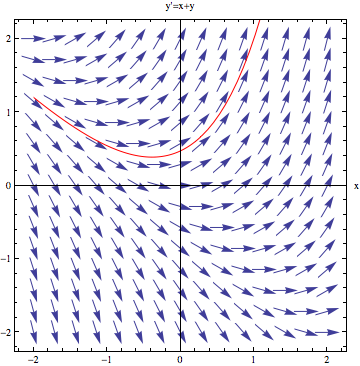
\includegraphics[width=.6\textwidth]{img/significato_geometrico_eq_diff.png}
	\end{figure}

	\noindent
	La ricerca delle primitive di una data funzione $f$, continua su un intervallo, equivale a risolvere l'equazione differenziale:
	\begin{equation*}
		y'=f\left(t\right)
	\end{equation*}
	che ha infinite soluzioni del tipo $y\left(t\right) = \displaystyle\int f\left(t\right) \:\mathrm{d}t + c, c \in \mathbb{R}$.

	Più in generale, l'\textbf{insieme delle soluzioni} di un'equazione differenziale di ordine $n$ o di un sistema di $n$ equazioni del primo ordine sia rappresentato da una famiglia di funzioni, \textbf{dipendente da $n$ parametri}. Tale famiglia prende il nome di \definition{integrale generale}.\newpage


	%%%%%%%%%%%%%%%%%%%%%%%%%%%%%%%%%%%%
	% Equazioni a variabili separabili %
	%%%%%%%%%%%%%%%%%%%%%%%%%%%%%%%%%%%%
	\subsection{Equazioni a variabili separabili}\label{subsection: equazioni a variabili separabili}

	Le \definition{equazioni a variabili separabili} sono della forma:
	\begin{equation}\label{eq: equazione a variabili separabili}
		y' = f\left(t\right)g\left(y\right)
	\end{equation}
	Con la funzione $f$ continua nell'intervallo $I$ ($f \in C\left(I\right)$) e la funzione $g$ continua nell'intervallo $J$ ($g \in C\left(J\right)$). Gli intervalli $I,J$ sono contenuti in $\mathbb{R}$.\newline

	\noindent
	\textbf{Nota bene:} se la funzione $\overline{y}$ è soluzione dell'equazione $g\left(y\right) = 0$, la retta $y = \overline{y}$ è una curva integrale (si veda l'esempio sottostante per convincersi di ciò).\newline

	\noindent
	Se $g\left(y\right) \ne 0$ in $J' \subseteq J$, l'integrale generale dell'equazione \ref{eq: equazione a variabili separabili} è:
	\begin{equation}\label{eq: integrale generale eq. a variabili separabili}
		\displaystyle\int \dfrac{1}{g\left(y\right)} \:\mathrm{d}y = \int f\left(t\right) \: \mathrm{d}t + c
	\end{equation}

	\begin{flushleft}
		\example{\underline{Esempio}}
	\end{flushleft}

	\noindent
	Data l'equazione:
	\begin{equation*}
		y' = 2t \sqrt{1-y^{2}}
	\end{equation*}
	Si può effettuare immediatamente un'osservazione importante. Come detto precedentemente, se $g\left(y\right) = 0$ e $\overline{y}$ è soluzione dell'equazione, allora $y = \overline{y}$ è una curva integrale. Si può facilmente trovare due valori di $y$ tali per cui l'equazione sia uguale a zero:
	\begin{equation*}
		\begin{array}{rcl}
			y = 1 & \longrightarrow & y' = 2t \sqrt{1 - 1^{2}} \\
				  &					& y' = 2 t \cdot 0 \\
				  &					& y' = 0 \\ [1em]
			y = -1& \longrightarrow & y' = 2t \sqrt{1 - \left(-1\right)^{2}} \\
				  & 				& y' = 2t \cdot 0 \\
				  &					& y' = 0
		\end{array}
	\end{equation*}
	Dato che:
	\begin{equation*}
		\begin{array}{rcl}
			f\left(t\right) &=& 2t \\
			g\left(y\right) &=& \sqrt{1-y^{2}}
		\end{array}
	\end{equation*}
	E con $y = \pm 1$ la funzione $g$ si annulla, allora $\pm 1$ sono soluzioni dell'equazione.\newline

	\noindent
	Adesso si cercano le soluzioni tali che $g\left(y\right) \ne 0$, quindi con $y \ne \pm 1$. Per farlo, si applica semplicemente la \dquotes{formula} \ref{eq: integrale generale eq. a variabili separabili}:
	\begin{equation*}
		\displaystyle\int \dfrac{1}{\sqrt{1-y^{2}}} \: \mathrm{d}y = 2 \displaystyle\int t \: \mathrm{d}t + c
	\end{equation*}
	Si procede con la risoluzione degli integrali:
	\begin{equation*}
		\begin{array}{rcl}
			\displaystyle 2 \cdot \int t \: \mathrm{d}t &=& 2 \cdot \dfrac{t^{2}}{2} = t^{2} + c \\ [2em]
			%
			\displaystyle \int \dfrac{1}{\sqrt{1 - y^{2}}} \: \mathrm{d}y & = & \arcsin\left(y\right) \\
		\end{array}
	\end{equation*}
	Si riaggregano i risultati:
	\begin{equation*}
		\arcsin\left(y\right) = t^{2} + c
	\end{equation*}
	Si esplicita la $y$ ricordando le proprietà della trigonometria $\arcsin\left(y\right) = x \rightarrow \sin\left(x\right) = y$:
	\begin{equation*}
		y = \sin\left(t^{2} + c\right)
	\end{equation*}
	


	\newpage

	%%%%%%%%%%%%%%%%%%%%%%
	% Problema di Cauchy %
	%%%%%%%%%%%%%%%%%%%%%%
	\subsection{Problema di Cauchy}\label{subsection: problema di Cauchy}

	Il \definition{problema di Cauchy (o dei valori iniziali)} ha due forme:
	\begin{itemize}
		\item Equazioni scalari di ordine $n$, con l'obbiettivo di trovare $y$ di classe\footnote{Con questa notazione si indica che una funzione ha una derivata continua di grado $n$. Quindi dicendo che $y$ è di classe $C^{4}$, vuol dire che $y$, $y'$, $y''$, $y'''$, $y''''$ sono tutte funzioni continue.} $C^{n}$ tale che:
		\begin{equation*}
			\begin{cases}
				y^{\left(n\right)}\left(t\right) = f\left(t, y\left(t\right), y'\left(t\right), ..., y^{\left(n-1\right)}\left(t\right)\right) \\
				%
				y\left(\tau\right) = \xi_{0} \\
				%
				y'\left(\tau\right) = \xi_{1} \\
				%
				\vdots 
				%
				y^{\left(n-1\right)}\left(\tau\right) = \xi_{n-1}
			\end{cases}
		\end{equation*}
		essendo $\tau, \xi_{0}, \cdots, \xi_{n-1}$ costanti assegnate;

		\item Sistemi, con l'obbiettivo di trovare $y$ di classe $C^{1}$ tale che:
		\begin{equation*}
			\begin{cases}
				y'=f\left(t, y\left(t\right)\right) \\
				y\left(\tau\right) = \xi
			\end{cases}
		\end{equation*}
		essendo $\tau \in \mathbb{R}$ e $\xi \in \mathbb{R}^{n}$ assegnati.
	\end{itemize}
	Le equazioni $y^{\left(j\right)}\left(\tau\right) = \xi_{j}$ con $j =0, \cdots, j=n-1$, e $y\left(\tau\right) = \xi$, prendono il nome di \definition{condizioni iniziali}. Le soluzioni si intendono definite localmente, ovvero in un intorno dell'istante iniziale $\tau$.\newline

	\noindent
	Un \example{esempio} di problema di Cauchy:
	\begin{equation*}
		\begin{cases}
			z''\left(t\right) + 4z'\left(t\right) + 4z\left(t\right) = \left(t+1\right)^{2} \\
			z\left(0\right) = \frac{1}{8} \\
			z'\left(0\right) = -3
		\end{cases}
	\end{equation*}

	\noindent
	Si consideri il seguente problema di Cauchy:
	\begin{equation*}
		(P)\begin{cases}
			y'\left(x\right) = a\left(x\right) b\left(y\right) \\
			y\left(x_{0}\right) = y_{0}
		\end{cases}
	\end{equation*}
	\begin{theorem}[\textbf{Teorema di esistenza e unicità locale per equazioni differenziabili a variabili separabili}]\label{theorem: teorema di esistenza e unicità locale per equazioni differenziabili a variabili separabili}
		Sia $a\left(x\right)$ una funzione continua in un intervallo aperto $I$ che contiene $x_{0}$ e $b\left(y\right)$ una funzione continua in un intervallo aperto $J$ che contiene $y_{0}$. Allora esiste $\delta > 0$ e una funzione definita per ogni $x \in I' \left[x_{0} - \delta, x_{0} + \delta\right] \subseteq I$ e ivi derivabile che risolve il problema di Cauchy. Se $b\left(y\right) \in C^{1}\left(J\right)$, allora tale soluzione unica.
	\end{theorem}

	\noindent
	Considerando il teorema \ref{theorem: teorema di esistenza e unicità locale per equazioni differenziabili a variabili separabili} enunciato poco fa, si intende dire che esiste almeno una funzione ($\overline{y}\left(x\right)$) tale che la sua derivata è uguale alla funzione continua ($a\left(x\right)$) moltiplicata per un'altra funzione continua ($b\left(y\right)$) che ha come parametro la primitiva:
	\begin{equation*}
		\begin{array}{rcl}
			\text{Primitiva} 	&\longrightarrow& \overline{y}\left(x\right) \\
			\text{Derivata}		&\longrightarrow& \overline{y}'\left(x\right) = a\left(x\right) \cdot b\left(\overline{y}\left(x\right)\right) \hspace{1em} \forall x \in \left[x_{0} - \delta, x_{0} + \delta \right]
		\end{array}
	\end{equation*}
	Ovviamente la derivata $\overline{y}\left(x\right)$ deve valere per qualsiasi $x$ che appartiene all'intorno $x_{0}$ aggiungendo/rimuovendo $\delta$. Inoltre la primitiva nel punto $x_{0}$ deve essere uguale a $y_{0}$ ($\overline{y}\left(x_{0}\right) = y_{0}$). Allora, la primitiva ($\overline{y}\left(x\right)$) è derivabile e la sua derivata è continua. L'unicità è possibile affermarla se la funzione $b\left(y\right)$ ha una proprietà più forte della continuità, ovvero la continuità nella derivata in $J$.

	\begin{boxdef}
		\definition{Teorema di esistenza e unicità globale per equazioni differenziali lineari.}\newline

		Si consideri l'equazione differneziale lineare
		\begin{equation*}
			y'\left(x\right) + a\left(x\right) \cdot y\left(x\right) = b\left(x\right)
		\end{equation*}
		Con $a\left(x\right)$ e $b\left(x\right)$ funzioni continue su un intervallo $I$ della retta reale. Se $x_{0} \in I$, allora il problema:
		\begin{equation*}
			\begin{cases}
				y'\left(x\right) + a\left(x\right) \cdot y\left(x\right) = b\left(x\right) & x \in I \\
				y\left(x_{0}\right) = y_{0}
			\end{cases}
		\end{equation*}
		Ammette un'unica soluzione in $I$.
	\end{boxdef}
	
	\begin{boxdef}
		\definition{Struttura dell'insieme delle soluzioni di un'equazione omogenea del primo ordine.}\newline

		L'insieme $V$ delle soluzioni dell'equazione omogenea
		\begin{equation*}
			y' + a\left(x\right)y = 0
		\end{equation*}
		È uno spazio vettoriale su $\mathbb{R}$ di dimensione $1$.

		Indicando con $y_{P}\left(x\right)$ una soluzione particolare dell'equazione completa
		\begin{equation*}
			y' + a\left(x\right) y = b\left(x\right)
		\end{equation*}
		Allora il suo integrale generale è
		\begin{equation*}
			y\left(x\right) = y_{P}\left(x\right) + y_{om}\left(x\right) \hspace{1em} y_{om}\left(x\right) \in V
		\end{equation*}
	\end{boxdef}\newpage

	\subsubsection{Intervallo massimale}\label{subsubsection: intervallo massimale}

	Si parte subito con il dire che determinare l'intervallo massimale non è un'operazione banale. Questo perché non esistono algoritmi (semplici) certi che consentono di ottenere un intervallo massimale. Tuttavia, lo studente può utilizzare il ragionamento ed eventuali intuizioni per capire quando una soluzione ha intervallo estendibile e quando esso è massimale.

	\begin{boxdef}
		Il più ampio intervallo su cui la soluzione è definita si chiama \definition{intervallo massimale}.
	\end{boxdef}

	\noindent
	L'intervallo massimale è possibile determinarlo una volta che si è giunti al termine del problema di Cauchy (par. \ref{subsection: problema di Cauchy}). Una volta concluso l'esercizio, avendo trovato l'integrale generale e la costante $c$, è necessario eseguire alcuni passaggi:
	\begin{enumerate}[label=\alph*)]
		\item Nell'integrale generale, sostituire la costante $c$ trovata al termine dell'esercizio;
		\item Esplicitare la $y$ tramite passaggi algebrici;
		\item Porre la condizione di esistenza;
		\item Studiare l'intervallo massimale con appositi ragionamenti.
	\end{enumerate}
	Si procede presentando due esempi e ricordando che un intervallo, \underline{\textbf{può}} essere esteso se rispetta certe condizioni.

	\begin{flushleft}
		\example{\underline{Esempio 1}}
	\end{flushleft}

	\noindent
	Dato il seguente problema di Cauchy:
	\begin{equation*}
		\begin{cases}
			y' = \sqrt{y}e^{-x} \\
			y\left(0\right) = 1
		\end{cases}
	\end{equation*}
	Calcolare l'intervallo massimale.\newline

	\noindent
	Il problema è risolvibile con il metodo delle variabili separabili (par. \ref{subsection: equazioni a variabili separabili}):
	\begin{equation*}
		\begin{array}{rcl}
			y'\left(x\right) &=& f\left(x\right) g\left(y\right) \\
			f\left(x\right) &=& e^{-x} \\
			g\left(y\right) &=& \sqrt{y} \\ [1em]
			\displaystyle\int \dfrac{1}{\sqrt{y}} \: \mathrm{d}y &=& \displaystyle\int e^{-x} \: \mathrm{d}x + c
		\end{array}
	\end{equation*}
	Si potrebbe tentare di calcolare una soluzione costante, ma risulterebbe evidente che l'unica soluzione costante, cioè $y = 0$, non è ammessa come soluzione del problema (condizione iniziale $y\left(0\right) = 1$!). Per questo motivo, si procede con il metodo delle variabili separabili.\newline

	\noindent
	Si risolve l'integrale:
	\begin{equation*}
		\begin{array}{rcl}
			\displaystyle\int y^{-\frac{1}{2}} \: \mathrm{d}y &=& -e^{-x} + c \\ [1em]
			%
			&\downarrow& \text{si utilizza l'integrale notevole } \displaystyle\int x^{n} \: \mathrm{d}x = \dfrac{x^{n+1}}{n+1} \hspace{1em} n \ne -1 \\ [1em]
			%
			\dfrac{y^{\frac{1}{2}}}{\dfrac{1}{2}} &=& -e^{-x} + c \\ [2.5em]
			%
			2\sqrt{y} &=& -e^{-x} + c
		\end{array}
	\end{equation*}
	La soluzione trovata è l'integrale generale. Si conclude il problema di Cauchy trovando la costante $c$, quindi applicando la condizione iniziale $y\left(0\right) = 1$:
	\begin{equation*}
		\begin{array}{rcl}
			2\sqrt{1} &=& -e^{-0} + c \\
			2 + 1 &=& c \\
			3 &=& c
		\end{array}
	\end{equation*}
	Adesso si calcola l'intervallo massimale:
	\begin{itemize}
		\item Si sostituisce nell'integrale generale la costante $c$:
		\begin{equation*}
			2\sqrt{y} = -e^{-x} + 3
		\end{equation*}
		Si esplicita la $y$:
		\begin{equation*}
			\begin{array}{rcl}
				\sqrt{y} &=& -\dfrac{e^{-x}}{2} + \dfrac{3}{2} \\ [.5em]
				y &=& \left(-\dfrac{e^{-x}}{2} + \dfrac{3}{2}\right)^{2}
			\end{array}
		\end{equation*}

		\item Le condizioni d'esistenza del problema di Cauchy sono le seguenti:
		\begin{equation*}
			\sqrt{y}e^{-x} \hspace{1em} \longrightarrow \hspace{1em} \underbrace{\left]-\infty, +\infty\right[}_{def. x} \times \overbrace{\left[0, +\infty \right[}^{def. y}
		\end{equation*}
		La $y$ deve essere maggiore/uguale a zero, mentre la $x$ non ha grosse restrizioni. L'intervallo massimale per definizione può essere identico o un sottoinsieme. Per trovarlo è necessario studiare il valore della $y$ esplicitata al passaggio precedente. In questo caso, essa in zero ($y=0$) non ha soluzione, per cui si cercano le soluzioni per $y > 0$.

		\item Andando a cercare una soluzione costante dell'equazione differenziale, ci si accorge che $g\left(y\right) = \sqrt{y}$ è uguale a zero solo se $y = 0$, e quindi essa sarebbe una soluzione costante del problema (ricordandosi quanto detto nel par. \ref{subsection: equazioni a variabili separabili}) poiché $g\left(y\right) = 0$ con $y = \overline{y}$. Tuttavia, $y = 0$ non è ammesso dal problema a causa della condizione iniziale $y\left(0\right) = 1$. 
		
		Per questo motivo, si cerca una soluzione tale che $y > 0$. E per farlo, si prende in considerazione la $y$ trovata al passaggio precedente e si impone una condizione:
		\begin{equation*}
			\begin{array}{rcl}
				-\dfrac{e^{-x}}{2} + \dfrac{3}{2} &>& 0 \\ [1em]
				-e^{-x} &>& -3 \\ [.3em]
				e^{-x} &<& 3 \\ [.3em]
				-x &<& \ln\left(3\right) \\ [.3em]
				x &>& -\ln\left(3\right)
			\end{array}
		\end{equation*}

		\item Per ciascun valore di $x$ che è maggiore di $-\ln\left(3\right)$, la $y$ deve valere:
		\begin{equation*}
			y = \left(-\dfrac{e^{-x}}{2} + \dfrac{3}{2}\right)^{2}
		\end{equation*}
		E per tutti gli altri casi? Nei casi in cui la $x$ sia minore o uguale a $-\ln\left(3\right)$, la $y$ dovrà valere $0$, come confermato nel caso della soluzione costante $y = 0$.

		Da queste considerazioni, è possibile rappresentare la soluzione del problema di Cauchy $\overline{y}$ come:
		\begin{equation*}
			\overline{y}\left(x\right) = \begin{cases}
				\left(-\dfrac{e^{-x}}{2} + \dfrac{3}{2}\right)^{2} 	& \text{se } x > -\ln\left(3\right) \\
				\\
				0													& \text{se } x \le -\ln\left(3\right)
			\end{cases}
		\end{equation*}
		Per cui l'intervallo massimale è $-\infty,+\infty$ e difatti si può estendere a destra e sinistra.
	\end{itemize}

	\begin{flushleft}
		\example{\underline{Esempio 2}}
	\end{flushleft}

	\noindent
	Dato il seguente problema di Cauchy:
	\begin{equation*}
		\begin{cases}
			y'-y^{2}\cos\left(x\right) = 0 \\
			\\
			y\left(\dfrac{\pi}{2}\right) = -1
		\end{cases}
	\end{equation*}
	Calcolare l'intervallo massimale.\newline

	\noindent
	Il problema è risolvibile con il metodo delle variabili separabili (par. \ref{subsection: equazioni a variabili separabili}):
	\begin{equation*}
		\begin{array}{rcl}
			y'\left(x\right) - f\left(x\right) g\left(y\right) &=& 0 \longrightarrow y'\left(x\right) = f\left(x\right) g\left(y\right) \\
			f\left(x\right) &=& \cos\left(x\right) \\
			g\left(y\right) &=& y^{2} \\ [1em]
			\displaystyle\int \dfrac{1}{y^{2}} \: \mathrm{d}y &=& \displaystyle\int \cos\left(x\right) \: \mathrm{d}x + c
		\end{array}
	\end{equation*}
	Si potrebbe tentare di calcolare una soluzione costante, ma risulterebbe evidente che l'unica soluzione costante, cioè $y = 0$, non è ammessa come soluzione del problema (condizione iniziale $y\left(\frac{\pi}{2}\right) = -1$!). Per questo motivo, si procede con il metodo delle variabili separabili.\newline

	\noindent
	Si risolve l'integrale:
	\begin{equation*}
		\begin{array}{rcl}
			\displaystyle\int \dfrac{1}{y^{2}} \: \mathrm{d}y &=& \displaystyle\int \cos\left(x\right) \: \mathrm{d}x \\ [1em]
			%
			\displaystyle\int y^{-2} \: \mathrm{d}y &=& \displaystyle\int \cos\left(x\right) \: \mathrm{d}x \\ [1em]
			%
			&\downarrow& \text{si utilizza l'integrale notevole } \displaystyle\int x^{n} \:\mathrm{d}x = \dfrac{x^{n+1}}{n+1} \hspace{1em} n \ne -1 \\ [1em]
			%
			\dfrac{y^{-1}}{-1} &=& \sin\left(x\right) \\ [1em]
			%
			-y^{-1} &=& \sin\left(x\right) \\ [.5em]
			%
			y &=& -\dfrac{1}{\sin\left(x\right)} + c
		\end{array}
	\end{equation*}
	La soluzione trovata è l'integrale generale. Si conclude il problema di Cauchy trovando la costante $c$, quindi applicando la condizione iniziale $y\left(\frac{\pi}{2}\right)=-1$:
	\begin{equation*}
		\begin{array}{rcl}
			-1 &=& -\dfrac{1}{\sin\left(\frac{\pi}{2}\right)} + c \\ [1em]
			%
			-1 &=& -\dfrac{1}{1} + c \\ [1em]
			%
			0 &=& c
		\end{array}
	\end{equation*}\newpage

	\noindent
	Adesso si calcola l'intervallo massimale:
	\begin{itemize}
		\item Si sostituisce nell'integrale generale la costante $c$:
		\begin{equation*}
			y = -\dfrac{1}{\sin\left(x\right)} + 0
		\end{equation*}
		
		\item La condizione d'esistenza del problema di Cauchy sono le seguenti:
		\begin{equation*}
			y^{2}\cos\left(x\right) \hspace{1em} \longrightarrow \hspace{1em} \underbrace{\left] -\infty, +\infty \right[}_{def. x} \times \overbrace{\left] -\infty, +\infty \right[}^{def. y}
		\end{equation*}

		\item A differenza dell'esempio precedente, in questo caso la $x$ non può essere qualsiasi valore poiché c'è un $\sin$ al denominatore che potrebbe causare una divisione per zero (impossibile). Per cui, la condizione d'esistenza è:
		\begin{equation*}
			\sin\left(x\right) > 0
		\end{equation*}
		Calcolando il $\arcsin$ di $0$, si ottiene:
		\begin{equation*}
			x > \arcsin\left(0\right) \longrightarrow x > 0
		\end{equation*}
		Ma attenzione! Perché il valore $\sin$ si può annullare anche con altri valori di $x$, come per esempio $\pi$, per cui:
		\begin{equation*}
			0 < x < \pi
		\end{equation*}
		Questo risulta l'intervallo massimale, ovviamente estremi esclusi.
	\end{itemize}\newpage

	\subsubsection{Equazioni differenziali lineari del secondo ordine}\label{subsubsection: equazioni differenziali lineari del secondo ordine}

	Le \definition{equazioni differenziali lineari del secondo ordine} nella forma standard sono composte nel seguente modo:
	\begin{equation*}
		y''\left(x\right) + a\left(x\right)y'\left(x\right) + b\left(x\right)y\left(x\right) = f\left(x\right)
	\end{equation*}
	Con $a\left(x\right)$, $b\left(x\right)$, $f\left(x\right) \in \mathcal{C}^{0}\left(I\right)$.\newline

	\noindent
	Il problema di Cauchy per una equazione lineare del secondo ordine è composto nel seguente modo:
	\begin{equation*}
		\begin{cases}
			y''\left(x\right) + a\left(x\right)y'\left(x\right) + b\left(x\right)y\left(x\right) = f\left(x\right) \\
			y\left(x_{0}\right) = y_{0} \\
			y'\left(x_{0}\right) = v_{0}
		\end{cases}
	\end{equation*}
	
	\begin{boxdef}
		\definition{Teorema di esistenza e unicità globale per equazioni lineari del secondo ordine.}\newline
		
		Si consideri l'equazione differenziale lineare
		\begin{equation*}
			y''\left(x\right) + a\left(x\right) \cdot y'\left(x\right) + b\left(x\right) \cdot y\left(x\right) = f\left(x\right)
		\end{equation*}
		Con $a\left(x\right)$, $b\left(x\right)$ e $f\left(x\right)$ funzioni continue su un intervallo $I$ detta retta reale. Se $x_{0} \in I$, allora il problema:
		\begin{equation*}
			\begin{cases}
				y''\left(x\right) + a\left(x\right)y'\left(x\right) + b\left(x\right)y\left(x\right) = f\left(x\right) \\
				y\left(x_{0}\right) = y_{0} \\
				y'\left(x_{0}\right) = v_{0}
			\end{cases}
		\end{equation*}
		Ammette un'unica soluzione in $I$.
	\end{boxdef}

	\begin{boxdef}
		\definition{Struttura dell'insieme delle soluzioni di un'equazione omogenea del secondo ordine}\newline

		L'insieme $V$ delle soluzioni di un'equazione differenziale lineare omogenea del secondo ordine è uno spazio vettoriale su $\mathbb{R}$ di dimensione $2$.
	\end{boxdef}

	\noindent
	L'insieme $S$ delle soluzioni dell'equazione completa è una varietà lineare:
	\begin{equation*}
		S = \left\{y_{P}\left(x\right) + y_{om}\left(x\right) : y_{om}\left(x\right) \in V\right\}
	\end{equation*}
	In cui $y_{P}\left(x\right)$ è una soluzione particolare dell'equazione completa.\newline

	\noindent
	Per risolvere questo tipo di equazioni, si utilizza il \textbf{metodo di somiglianza o dei coefficienti indeterminati} (par. \ref{subsection: metodo di somiglianza o dei coefficienti indeterminati}).\newpage

	\subsection{Metodo di somiglianza o dei coefficienti indeterminati}\label{subsection: metodo di somiglianza o dei coefficienti indeterminati}
	Il metodo di somiglianza o dei coefficienti indeterminati è una tecnica che consente di risolvere le equazioni differenziali lineari del secondo ordine rapidamente.\\

	\noindent
	Non esiste un'unica tecnica risolutiva, ma è necessario avere a disposizione una serie di \textbf{\emph{pattern risolutivi}}. Il motivo è dovuto al fatto che ogniqualvolta si presenti un'equazione differenziale lineare del secondo grado, si eseguirà un \emph{matching} tra i \emph{pattern risolutivi} che si hanno a disposizione e l'equazione risultante (in parole povere, l'espressione a destra dell'uguale).\newline

	\begin{table}[!htp]
		\centering
		\begin{tabular}{@{} l l l @{}}
			\toprule
			\textbf{Tipo}	& \textbf{Equazione differenziale} & \textbf{Soluzione particolare} \\
			\midrule
			Monomio	& $y'' + y' - 2y = 5$ & $y_{P}\left(x\right) = a$ \\
			\cmidrule{1-3}
			Primo grado 	& $y'' + y' - 2y = x + 2$ & $y_{P}\left(x\right) = ax + b$ \\ 
			\cmidrule{1-3} 
			Secondo grado	& $y'' + 3y' + 2y = 2x^{2} - 1$ & $y_{P}\left(x\right) = ax^{2} + bx + c$ \\
			\cmidrule{1-3} 
			\multirow{4}{*}{Esponenziale} 	& $y'' + 3y' - 2y = 3e^{-x}$	& $y_{P}\left(x\right) = ae^{-x}$ \\ [.3em]
			& $y'' - 3y' + 2y = 3e^{-x} \cdot x$	& $y_{P}\left(x\right) = \left(ax + b\right) e^{-x}$ \\ [.3em]
			& $y'' - 3y' + 2y = 3e^{x}$	& $y_{P}\left(x\right) = x \cdot ae^{x}$ \\ [.3em]
			& $y'' - 3y' + 2y = 3e^{2x} \cdot x$	& $y_{P}\left(x\right) = \left(ax + b\right) e^{2x} \cdot x$ \\
			\cmidrule{1-3}
			Coseno/Seno 	& $y'' + y' = \cos\left(2x\right)$ & $y_{P}\left(x\right) = a \cdot \cos\left(2x\right) + b \cdot \sin\left(2x\right)$ \\
			\bottomrule
		\end{tabular}
		\caption{Pattern risolutivi del metodo di somiglianza.}
		\label{tab: pattern risolutivi del metodo di somiglianza}
	\end{table}

	\noindent
	A questi pattern è necessario aggiungere alcuni casi che modificano la soluzione particolare. \textbf{Attenzione:} questi casi modificano la soluzione particolare scelta! Nella tabella \ref{tab: casi particolari del metodo di somiglianza}, si indicano con $\lambda$ le soluzioni dell'equazione caratteristica (in parole povere l'equazione a sinistra dell'uguale).\newline

	\noindent
	Un altro caso particolare è il \textbf{principio di sovrapposizione}. In questo caso, basta risolvere ogni fattore come un'equazione a sé stante. Per cui la soluzione particolare si compone nel seguente modo:
	\begin{equation*}
		y_{P}\left(x\right) = y_{P_{1}}\left(x\right) + y_{P_{2}}\left(x\right)
	\end{equation*}
	Per esempio, data l'equazione:
	\begin{equation*}
		y'' + 6y' + 8y = e^{2x} + \sqrt{\pi} x^{2}
	\end{equation*}
	Si risolve:
	\begin{equation*}
		y'' + 6y' + 8y = e^{2x}
	\end{equation*}
	E successivamente:
	\begin{equation*}
		y'' + 6y' + 8y = \sqrt{\pi} x^{2}
	\end{equation*}\newpage

	\begin{table}[!htp]
		\centering
		\begin{tabular}{@{} c c c @{}}
			\toprule
			$\boldsymbol{\lambda}$ & \textbf{Equazione differenziale} & \textbf{Che cosa viene modificato} \\
			\midrule
			%
			\multicolumn{3}{p{32em}}{\framedtext{Nel caso in cui la soluzione dell'equazione caratteristica è uguale a zero, si moltiplica la \textbf{soluzione particolare} per $x$. Quest'ultima viene elevata ad un valore pari al numero di volte che essa annulla l'equazione caratteristica.
			
			Nell'esempio sottostante, la $x$ viene elevata ad $1$ poiché le soluzioni dell'equazione caratteristica sono $\lambda_{1} = 0$ e $\lambda_{2} = -1$. Dunque, $\lambda_{1}$ annulla soltanto una volta l'equazione caratteristica (chiamata formalmente molteplicità algebrica).
			
			\underline{Attenzione:} la regola viene applicata solo ai polinomi di primo e secondo grado.}}\\\\
			$\lambda = 0$ & $y''+y' = x+2$ & $y_{P}\left(x\right) = \left(ax+b\right)x^{1}$ \\ [.5em]
			%
			\cmidrule{1-3}
			%
			\multicolumn{3}{p{32em}}{\framedtext{Nel caso in cui le soluzioni dell'equazione caratteristica siano uguale tra di loro, si modifica la \textbf{soluzione generale} aggiungendo una $x$.
			
			Nell'esempio sottostante, le soluzioni dell'equazione caratteristica sono $\lambda_{1} = \lambda_{2} = 1$ per cui viene aggiunta una $x$ nella soluzione generale.}} \\\\
			$\lambda_{1} = \lambda_{2}$ & $y'' - 2y' + y = \left(x - 1\right)^{2}$ & $y\left(x\right) = y_{P}\left(x\right) + c_{1}e^{x} + c_{2}e^{x} \cdot x$ \\ [.5em]
			%
			\cmidrule{1-3}
			%
			\multicolumn{3}{p{32em}}{\framedtext{Nel caso in cui le soluzioni dell'equazione caratteristica siano uguali al termine dell'esponenziale ($e^{\alpha x}$) presente a destra dell'uguale dell'equazione caratteristica, alla \textbf{soluzione particolare} viene moltiplicata una $x$ elevata ad un valore pari alla sua molteplicità algebrica.
			
			Nell'esempio sottostante, le soluzioni dell'equazione caratteristica sono $\lambda_{1} = $ e $\lambda_{2} = $. E dato che il valore di $\lambda_{n}$ compare nell'esponenziale dell'equazione caratteristica, viene aggiunta una $x$.
			
			\underline{Attenzione:} la regola vale solo se l'esponenziale ha una $x$ tra i suoi termini, quindi non è valida per esempio con $e^{2}$. In generale deve essere: $e^{\alpha x}$}} \\\\
			$\lambda_{1} = \alpha$ & $y'' - 5y' + 6y = 3x e^{2x}$ & $y_{P}\left(x\right) = x \cdot \left[e^{2x}\left(ax+b\right)\right]$ \\ [.5em]
			%
			\cmidrule{1-3}
			%
			\multicolumn{3}{p{32em}}{\framedtext{Nel caso in cui le soluzioni dell'equazione caratteristica siano numeri immaginari e uguali: al termine dell'esponenziale ($e^{\alpha x}$) e al termine del seno/coseno ($\cos\left(\beta x\right)$/$\sin\left(\beta x\right)$); allora viene aggiunta una $x$ alla \textbf{soluzione particolare}.}} \\\\
			\multirow{2}{*}{$\lambda = \alpha \pm \beta i$} & $y'' \cdots = e^{\alpha x} \cos\left(\beta x\right)$ & \multirow{2}{*}{$y_{P}\left(x\right) = x \cdot e^{\alpha x}\left(\cos\left(\beta x\right) + \sin\left(\beta x\right)\right)$} \\
			& $y'' \cdots = e^{\alpha x} \sin\left(\beta x\right)$ & \\
			\bottomrule
		\end{tabular}
		\caption{Casi particolari della $\lambda$ nel metodo di somiglianza.}
		\label{tab: casi particolari del metodo di somiglianza}
	\end{table}\newpage

	% TODO: add examples

	\subsection{Metodo di variazione delle costanti}

	Il \definition{metodo di variazione} delle costanti è una tecnica più generale che consente di ricavare una soluzione particolare dell'equazione completa, qualunque sia la forma del termine forzante (cioè quello a destra dell'uguale).\newline

	\noindent
	Data l'equazione differenziale lineare del secondo ordine:
	\begin{equation*}
		y'' + ay' + by = f\left(x\right)
	\end{equation*}
	Dopo aver ottenuto la soluzione particolare con il metodo di somiglianza (par. \ref{subsection: metodo di somiglianza o dei coefficienti indeterminati}):
	\begin{equation*}
		y_{P}\left(x\right) = c_{1}\left(x\right)y_{1}\left(x\right) + c_{2}\left(x\right) y_{2}\left(x\right)
	\end{equation*}
	Si possono ottenere le due costanti grazie a queste operazioni tra matrici:
	\begin{equation*}
		\underbrace{
			\begin{bmatrix}
				y_{1}\left(x\right) & y_{2}\left(x\right) \\
				y_{1}'\left(x\right) & y_{2}'\left(x\right)
			\end{bmatrix}
		}_{Wronskiana}
		\cdot
		\begin{bmatrix}
			c_{1}'\left(x\right) \\
			c_{2}'\left(x\right)
		\end{bmatrix}
		=
		\begin{bmatrix}
			0 \\
			f\left(x\right)
		\end{bmatrix}
	\end{equation*}
	Attenzione, in questo caso le costanti sono derivate, per cui è necessario integrarle per ottenere la soluzione finale.

	\begin{flushleft}
		\example{\underline{\textbf{Esempio}}}
	\end{flushleft}

	\noindent
	Determinare l'integrale generale dell'equazione:
	\begin{equation*}
		y'' + y = \sin\left(x\right)
	\end{equation*}
	Le soluzioni dell'equazione caratteristica sono:
	\begin{equation*}
		\dfrac{-0 \pm \sqrt{0^{2} - 4 \cdot 1 \cdot 1}}{2} = \dfrac{\pm\sqrt{-4}}{2} = \dfrac{\pm2i}{2} = \pm i
	\end{equation*}
	La soluzione generale dunque è:
	\begin{equation*}
		y\left(x\right) = y_{P}\left(x\right) + c_{1} e^{i \cdot x} + c_{2} e^{-i \cdot x}
	\end{equation*}
	Per ottenere la soluzione particolare viene utilizzato il metodo di somiglianza:
	\begin{equation*}
		y_{P}\left(x\right) = a \cdot \cos\left(x\right) + b \cdot \sin\left(x\right)
	\end{equation*}
	Adesso viene utilizzato il metodo di variazione per ottenere le costanti. Quindi si costruiscono le matrici:
	\begin{equation*}
		\begin{array}{rcl}
			\begin{bmatrix}
				y_{1}\left(x\right) & y_{2}\left(x\right) \\
				y_{1}'\left(x\right) & y_{2}'\left(x\right)
			\end{bmatrix}
			\cdot
			\begin{bmatrix}
				a'\left(x\right) \\
				b'\left(x\right)
			\end{bmatrix}
			&=&
			\begin{bmatrix}
				0 \\
				f\left(x\right)
			\end{bmatrix} \\ [1em]
			%
			\begin{bmatrix}
				\cos\left(x\right) & \sin\left(x\right) \\
				-\sin\left(x\right) & \cos\left(x\right)
			\end{bmatrix}
			\cdot
			\begin{bmatrix}
				a' \\ b'
			\end{bmatrix}
			&=&
			\begin{bmatrix}
				0 \\ \sin\left(x\right)
			\end{bmatrix} \\ [.8em]
			%
			\begin{bmatrix}
				a' \\ b'
			\end{bmatrix}
			&=&
			\begin{bmatrix}
				\cos\left(x\right) & -\sin\left(x\right) \\
				\sin\left(x\right) & \cos\left(x\right)
			\end{bmatrix}^{-1}
			\cdot
			\begin{bmatrix}
				0 \\ \sin\left(x\right)
			\end{bmatrix} \\ [1em]
			%
			\begin{bmatrix}
				a' \\ b'
			\end{bmatrix}
			&=&
			\begin{bmatrix}
				- \sin^{2}\left(x\right) \\
				\cos\left(x\right) \sin\left(x\right)
			\end{bmatrix}
		\end{array}
	\end{equation*}\newpage

	\noindent
	Per ottenere le costanti $a$ e $b$ è necessario integrare le derivate appena trovare, per cui:
	\begin{equation*}
		\begin{array}{rcl}
			a &=& \displaystyle\int -\sin^{2}\left(x\right) \:\mathrm{d}x \\
			%
			&\downarrow& \text{si utilizza l'integrale fondamentale } \displaystyle\int \sin^{2}\left(x\right) \: \mathrm{d}x = \int\dfrac{1-\cos\left(2x\right)}{2} \: \mathrm{d}x \\ [1em]
			%
			&=& - \displaystyle\int \dfrac{1-\cos\left(2x\right)}{2} \:\mathrm{d}x \\ [1em]
			%
			&=& -\displaystyle\int \dfrac{1}{2} - \dfrac{\cos\left(2x\right)}{2} \:\mathrm{d}x \\ [1em]
			%
			&=& \displaystyle -\left( \int\dfrac{1}{2} \:\mathrm{d}x - \int \dfrac{\cos\left(2x\right)}{2} \:\mathrm{d}x \right) \\ [1em]
			%
			&=& \displaystyle -\left( \dfrac{1}{2}x - \dfrac{1}{2}\cdot\int\cos\left(2x\right) \:\mathrm{d}x \right) \\ [1em]
			%
			&\downarrow& \text{si ricorda il risultato della seguente derivata } \dfrac{\mathrm{d}}{\mathrm{d} x} \sin\left(5x\right) = 5\cos\left(5x\right) \\ [1em]
			%
			&=& -\dfrac{1}{2}x -\left(-\dfrac{1}{2} \cdot \dfrac{\sin\left(2x\right)}{2}\right) \\ [1em]
			%
			&=& -\dfrac{1}{2}x + \dfrac{\sin\left(2x\right)}{4} \\ [3em]
			%
			%~~~~~~~~~~~~~~~~~~~~~~~~~~~~~~~~~~~~~~~~~~%
			%
			b &=& \displaystyle\int \cos\left(x\right)\sin\left(x\right) \: \mathrm{d}x \\
			%
			&\downarrow& \text{si utilizza il metodo di sostituzione } t = \sin\left(x\right) \hspace{1em} \mathrm{d}x = \dfrac{1}{t'} \: \mathrm{d}t \\ [1em]
			%
			&=& \displaystyle\int \cos\left(x\right) \cdot t \cdot \dfrac{1}{\cos\left(x\right)} \: \mathrm{d}t \\ [1em]
			%
			&=& \displaystyle\int \cancel{\cos\left(x\right)} \cdot t \cdot \dfrac{1}{\cancel{\cos\left(x\right)}} \: \mathrm{d}t \\ [1em]
			%
			&=& \displaystyle\int t \: \mathrm{d}t \\ [1em]
			%
			&=& \dfrac{t^{2}}{2} \\ [1em]
			%
			&\downarrow& \text{si conclude il metodo di sostituzione} \\ [1em]
			%
			&=& \dfrac{\sin^{2}\left(x\right)}{2} + c
		\end{array}
	\end{equation*}
	Per cui, andando a sostituire i due risultati nella soluzione particolare, è possibile ottenere anche la soluzione generale:
	\begin{gather*}
		\begin{array}[pos]{rcl}
			y_{P}\left(x\right) &=& \left(-\dfrac{1}{2}x + \dfrac{\sin\left(2x\right)}{4}\right)\cos\left(x\right) + \left(\dfrac{\sin^{2}\left(x\right)}{2}\right)\sin\left(x\right) \\ [1.4em]
			%
			y\left(x\right) &=& y_{P}\left(x\right) + c_{1} e^{i \cdot x} + c_{2} e^{-i \cdot x}
		\end{array}
	\end{gather*}
	% TODO: slides 6, end differential equations
\end{document}